% ============================================================================
% PAQ-KV — AAAI-27 submission draft, distilled from paq_living.tex (2026-07-17).
% Every number is taken verbatim from the living document; nothing re-derived.
% 2026-07-22 style revision (v2): prose reworked to match AB's register
% (no em dashes, no "beat" vocabulary, plain section titles); all numbers,
% tables, labels and citations unchanged.
% 2026-07-24: PAQ acronym defined (Prefill once, Ask many Queries); page-level
% labelling clarified; duplicate Figure 2 include removed (long caption kept);
% \ref{sec:limitations} retargeted to app:repro after that section was
% commented out (collaborator pass). Table 1 LongDocURL vs-full/vs-oracle
% contrasts filled from research/paqc_topup_fulloracle_posthoc.json (post-hoc,
% identical frozen instrument; replaces an unbacked "(n.s.)" and an "n/a").
% 2026-07-25: cross-reader generality folded in from the internal companion
% note (paq_cross_reader_generality.tex): new \S Results subsection
% sec:results-crossreader + Table tab:crossreader (numbers verbatim from the
% companion's tab:main/tab:longdocurl + InternVL frontier; the Qwen3-VL-8B row
% repeats Table 1's verified values, NOT the companion's 0.3284/+0.076 variant);
% abstract, evidence-status, setup single-reader sentence, and conclusion
% updated accordingly; eviction-family pointer added to \S5.2.
% 2026-07-26: AAAI framing pass (external AAAI-format review applied): abstract
% cut to ~205 words; contributions -> three short bullets; Evidence Status moved
% to \S Setup; \S3.3 audit detail -> app:reversibility; \S4.4 integrity
% narratives -> app:integrity (summary kept); Results reorganized around
% questions (5.1 re-selection, 5.2 vs trained retrieval, 5.3 scope incl.
% cross-reader, 5.4 systems); tab:contrasts + tab:crossreader + negatives +
% second-reader baseline prose -> appendix; NEW Figure fig:forest
% (figures/fig_forest_contrasts.pdf, seaborn, scripts/make_fig_forest_contrasts.py,
% values transcribed from verdict-backed tex numbers) replaces both tables in
% the main text; systems framing made neutral (no "honest summary runs against
% us"); appendix regrouped into 4 thematic sections (A impl/repro, B complete
% results, C additional analyses, D limitations) with all previous labels kept.
% Metric scale left at 0-1 (NOT x100) to stay consistent with the generated,
% script-produced tables (nothing hand-entered); revisit only via the
% generation scripts. Figure 3 (framework.pdf) kept per collaborator graphics
% pass despite overlap with Figure 2. All numbers verbatim; nothing re-derived.
% Build: ./tectonic -X compile paq_aaai.tex
% ============================================================================
\documentclass[letterpaper]{article} % DO NOT CHANGE THIS
% ---------------------------------------------------------------------------
% LOCAL BUILD SHIM (this block only; the style file itself is untouched):
% the host has no pdflatex, so this draft is built with tectonic (XeTeX-based).
% aaai2027.sty's engine guard (\RequirePDFTeX) is neutralized ONLY when the
% engine is not pdfTeX. Under the official pdflatex build this block is inert
% and the guard runs as shipped. Remove the shim for the actual submission.
\usepackage{iftex}
\ifPDFTeX\else\let\RequirePDFTeX\relax\fi
% ---------------------------------------------------------------------------
\usepackage[submission]{aaai2027}  % DO NOT CHANGE THIS
\usepackage[hyphens]{url}  % DO NOT CHANGE THIS
\usepackage{graphicx} % DO NOT CHANGE THIS
\urlstyle{rm} % DO NOT CHANGE THIS
\def\UrlFont{\rm}  % DO NOT CHANGE THIS
\usepackage{natbib}  % DO NOT CHANGE THIS AND DO NOT ADD ANY OPTIONS TO IT
\usepackage{caption} % DO NOT CHANGE THIS AND DO NOT ADD ANY OPTIONS TO IT
\frenchspacing  % DO NOT CHANGE THIS
\usepackage{algorithm}
\usepackage{algorithmic}
\usepackage{booktabs}
\usepackage{multirow}
\usepackage{amsmath}
\usepackage{amssymb}


\pdfinfo{
/TemplateVersion (2027.1)
}

\setcounter{secnumdepth}{2}

\graphicspath{{figures/}}

\newcommand{\paq}{\textsc{PAQ}}
\newcommand{\paqt}{\textsc{PAQ-T}}
\newcommand{\paqc}{\textsc{PAQ-KV}}
\newcommand{\lb}{\mathrm{LB}_{95}}
% Below-page isolation-gate numbers, generated by BASED/scripts/paq_isogate_tex.py from
% research/paq_isogate_kv_verdict.json (2026-07-26 run; nothing hand-entered).
% GENERATED by scripts/paq_isogate_tex.py 2026-07-26 10:54 — DO NOT EDIT BY HAND
% source: research/paq_isogate_kv_verdict.json (pin research/paq_confirm_pin.json sha 01f4e203ec67c2d5; n_complete=907/907; verdict=REVERSIBILITY_ISOLATED_BELOWPAGE)

\newcommand{\isoKVLduCommitDelta}{+0.211}
\newcommand{\isoKVLduCommitLb}{+0.136}
\newcommand{\isoKVLduCommitUb}{+0.289}
\newcommand{\isoKVLduCommitCI}{[+0.136,+0.289]}
\newcommand{\isoKVLduStaticDelta}{+0.230}
\newcommand{\isoKVLduStaticLb}{+0.178}
\newcommand{\isoKVLduStaticUb}{+0.276}
\newcommand{\isoKVLduStaticCI}{[+0.178,+0.276]}
\newcommand{\isoKVLduFresh}{0.531}
\newcommand{\isoKVLduCommitAcc}{0.320}
\newcommand{\isoKVLduStaticAcc}{0.301}
\newcommand{\isoKVLduNc}{463}
\newcommand{\isoKVLduNdocs}{80}
\newcommand{\isoKVMmCommitDelta}{+0.137}
\newcommand{\isoKVMmCommitLb}{+0.103}
\newcommand{\isoKVMmCommitUb}{+0.169}
\newcommand{\isoKVMmCommitCI}{[+0.103,+0.169]}
\newcommand{\isoKVMmStaticDelta}{+0.213}
\newcommand{\isoKVMmStaticLb}{+0.160}
\newcommand{\isoKVMmStaticUb}{+0.266}
\newcommand{\isoKVMmStaticCI}{[+0.160,+0.266]}
\newcommand{\isoKVMmFresh}{0.405}
\newcommand{\isoKVMmCommitAcc}{0.268}
\newcommand{\isoKVMmStaticAcc}{0.192}
\newcommand{\isoKVMmNc}{444}
\newcommand{\isoKVMmNdocs}{80}
\newcommand{\isoKVPoolCommitDelta}{+0.174}
\newcommand{\isoKVPoolCommitLb}{+0.132}
\newcommand{\isoKVPoolCommitCI}{[+0.132,+0.215]}
\newcommand{\isoKVPoolStaticDelta}{+0.221}
\newcommand{\isoKVPoolStaticLb}{+0.184}
\newcommand{\isoKVPoolStaticCI}{[+0.184,+0.256]}
\newcommand{\isoKVNComplete}{907}
\newcommand{\isoKVNPinned}{907}
\newcommand{\isoKVNIncomplete}{0}
\newcommand{\isoKVVerdict}{met}


\newcommand{\jiahui}[1]{\textcolor{red}{[Jiahui: #1]}}

\title{Prefill Once, Ask Many: Training-Free Reversible Below-Page KV Selection\\for Multi-Query Long-Document Visual Question Answering}
\author{
    Anonymous submission
}
\affiliations{
    Anonymous submission
}

\begin{document}

\maketitle

\begin{abstract}
Long-document visual question answering is naturally multi-query: a document
is read once, but successive questions need different evidence. Existing
KV-cache eviction methods commit to one compressed context, so evidence
discarded for the first question is unavailable to later ones. We present
\paqc{} (``Prefill once, Ask many Queries''), a training-free method that
prefills a document once, retains its complete KV cache, and constructs a new
query-specific attention view for every question: the frozen reader's own
question-to-context attention scores 64-token page-aligned blocks, and
decoding applies a four-dimensional additive mask that exposes only the
selected blocks at their original M-RoPE positions. Because the cache is
neither gathered nor evicted, every selection is reversible, with no
additional model, retrieval index, or document re-read. At a nominal 5\%
decode-attention budget (${\approx}6\%$ realized), \paqc{} scores $0.404$ on
MMLongBench-Doc versus $0.328$ for the trained ColQwen2 retriever, and a
disjoint sealed test set evaluated exactly once under a frozen protocol
confirms the improvement ($+0.076$, document-clustered 95\% CI
$[+0.029,+0.122]$). Per-query re-selection also outperforms committing the
identical scorer once, by wide margins. Further datasets and readers bound
the scope: the advantage is largest where evidence is dispersed and the host
reader's attention localizes it well, and reverses on a retrieval-native cell
and on InternVL3.5-8B.
\end{abstract}

\section{Introduction}\label{sec:intro}

% Figure source: BASED/research/paq_sealed_final_sealed_verdict.json
\begin{figure}[t]
\centering
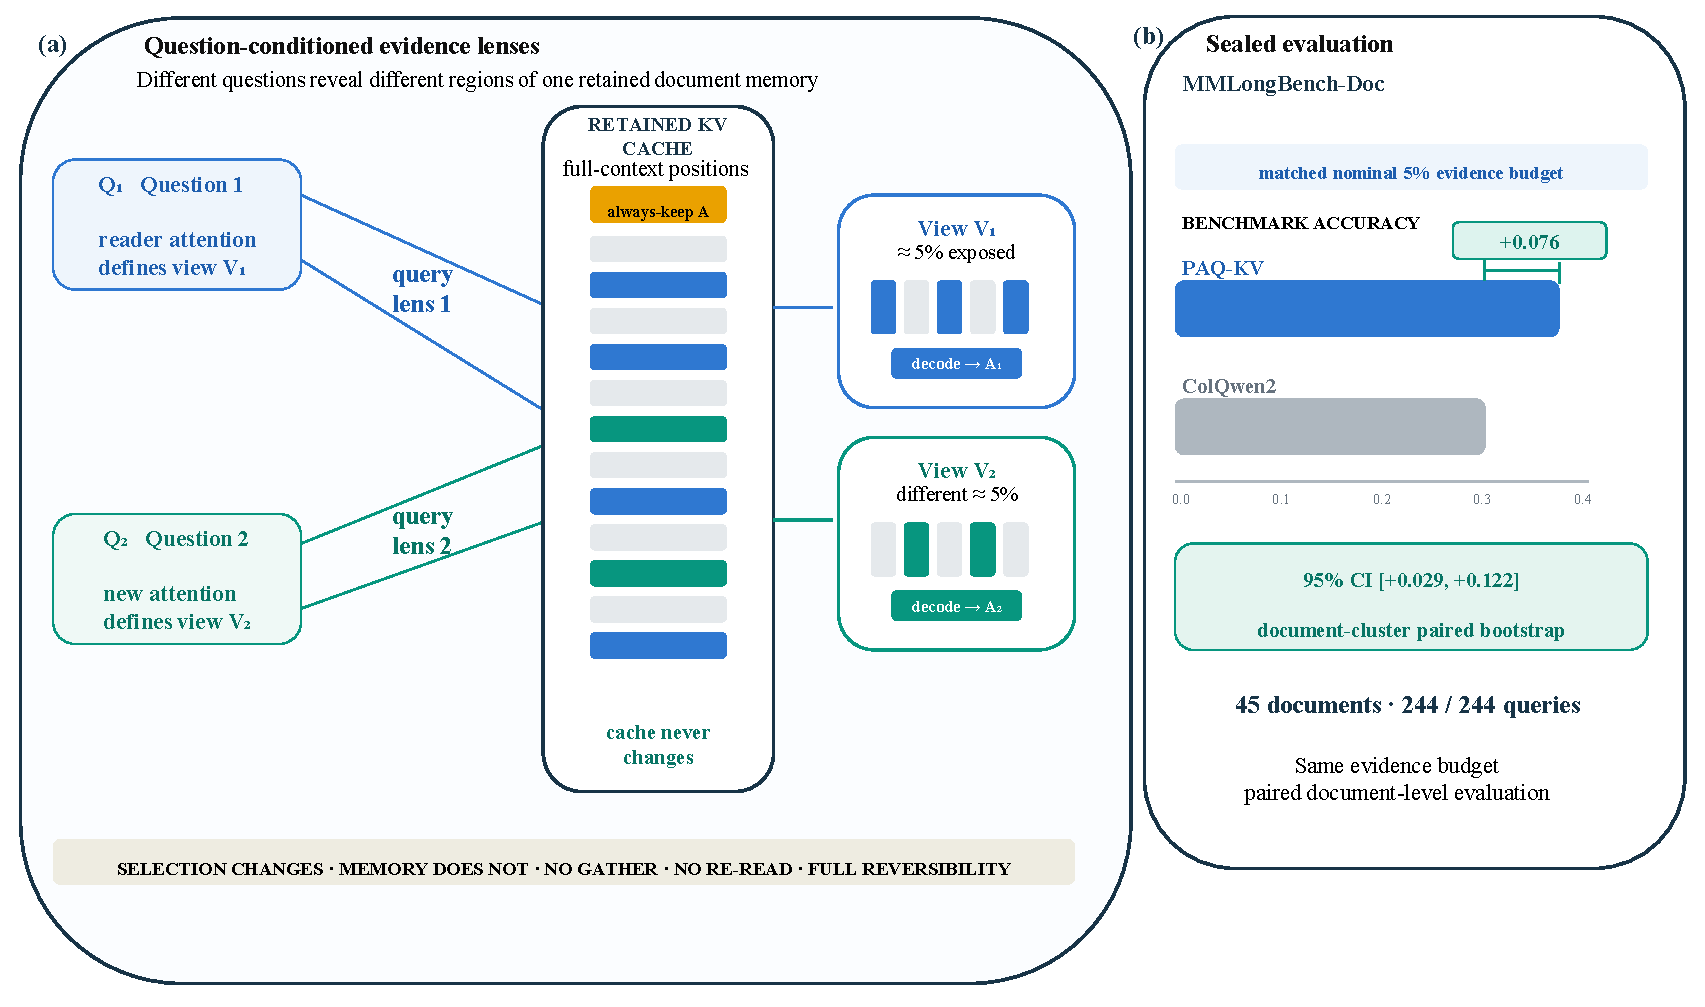
\includegraphics[width=\columnwidth]{figures/figure1_variant_b_evidence_lenses_editable.pdf}
% Coauthor note (was inline \jiahui in the caption): this figure is too close
% to Figure 2, need to change.
\caption{Method and sealed result at a glance. On fresh, disjoint MMLongBench-Doc, \paqc{}@5\% scores $0.396$ versus $0.320$ for corrected-loader ColQwen2 ($+0.076$, document-clustered 95\% CI $[+0.029,+0.122]$; 45 documents, 244/244 queries).}
\label{fig:overview}
\end{figure}

Long-context vision-language models (VLMs) can read an entire multi-page document, but they pay for every page on every question. The standard efficiency response, inherited from single-query text benchmarks, is to \emph{evict}: after reading, the model keeps only a compact subset of its KV cache, the stored per-token state that decoding attends to, and discards the rest \citep{li2024snapkv,zhang2023h2o,chen2024fastv,wan2024lookm,kim2025kvzip}. Eviction is a single, irreversible commitment: whatever subset survives must serve every future question about that document.

In practice, however, document assistants are not asked one question. Both benchmarks in this study, MMLongBench-Doc \citep{ma2024mmlongbench} and LongDocURL \citep{deng2025longdocurl}, pose long-document visual question answering (VQA) natively as groups of questions about a shared document. Inside our pinned evaluation subsets the average document carries more than five gold-bearing questions (\S\ref{sec:setup}). Different questions need different evidence, so a subset committed for question~1 is stale by question~5.

This paper asks two questions. At a matched evidence budget on long multimodal
documents, does \emph{re-selecting} context for every query beat selecting once
and committing? And can a training-free selector built from the reader's own
internals compete with a dedicated trained retriever? Our answer is \paqc{}
(Prefill once, Ask many Queries).

\paqc{} works as follows. A frozen reader (Qwen3-VL-8B; \citealp{qwen3vl2025})
prefills the document once and keeps the resulting KV cache. Each question is
then scored against that cache by the reader's own attention from the question
tokens to the document tokens, and those scores rank the cache's 64-token
blocks. Blocks are the granularity below the page: a typical page spans several
of them, so a block is roughly a table row, a figure caption, or a paragraph
rather than a whole page of mixed content. The answer is decoded from the full
cache under a four-dimensional attention mask that exposes only the top-ranked
blocks. Nothing is gathered and nothing is discarded, so every position index
stays the model's own. This matters because the reader family indexes tokens
with M-RoPE \citep{bai2025qwen25vl}, a multimodal rotary position embedding that
gives an image token its temporal, height, and width coordinates on the page
rather than a flat sequence offset; physically compacting the cache would have
to reassign these composite indices, while leaving it in place avoids the
question entirely. Each selection is therefore \emph{reversible}: the next
question re-selects from the same intact cache. Figure~\ref{fig:overview}
summarizes the architecture and its sealed MMLongBench-Doc result.

\paragraph{Contributions.}
\begin{itemize}
\item \textbf{A reversible, training-free selection architecture.} \paqc{}
retains the full-document KV cache and gives every query its own below-page
selection through a per-query 4D additive decode mask, preserving native
M-RoPE positions with no gathering, eviction, or re-read (\S\ref{sec:method}).
\item \textbf{A pre-registered isolation of reversibility.} Holding the
scorer and budget fixed, per-query re-selection outperforms the same scorer
committed once by $\isoKVMmCommitDelta$/$\isoKVLduCommitDelta$
(MMLongBench-Doc/LongDocURL) and a gold-informed static subset by
$\isoKVMmStaticDelta$/$\isoKVLduStaticDelta$, with document-clustered
intervals excluding zero in every cell (\S\ref{sec:results-isolation}).
\item \textbf{An out-of-sample-confirmed improvement over a trained
retriever, with its scope measured.} At a matched 5\% budget \paqc{}
outperforms ColQwen2 by $+0.077$ on MMLongBench-Doc, confirmed once on a
sealed disjoint set ($+0.076$); MMDocRAG reproduces the improvement, a
retrieval-native MMDocIR cell reverses it, LongDocURL is a statistical tie,
and a full-method port to three further readers bounds generality
(\S\ref{sec:results}).
\end{itemize}

\section{Related Work}\label{sec:related}

\paragraph{Page selection and retrieval.} CAPS \citep{zhu2026caps} publishes
attention-based \emph{page} selection on our benchmarks, and ColPali/ColQwen2
\citep{faysse2025colpali} are the strongest trained retrieval baselines we
compare against. Selecting pages with reader attention is CAPS's method; \paqc{}
differs on the axes CAPS names as open. It selects below the page, it re-selects
per query over a single retained prefill rather than committing once, and it
decodes directly from the retained cache with no re-read.

\paragraph{KV-cache eviction.} SnapKV \citep{li2024snapkv}, H2O
\citep{zhang2023h2o}, FastV \citep{chen2024fastv}, LOOK-M \citep{wan2024lookm},
and KVzip \citep{kim2025kvzip} all commit a compressed cache once. Quest
\citep{tang2024quest} shows that query-aware selection can outperform
query-agnostic eviction in single-query text, which motivates but does not prove
our multi-query claims. We did not find prior work that combines reader-internal
attention as the runtime below-page selector, end-to-end question answering at a
matched budget against page-level retrieval, and long multi-query documents; we
offer this as a provisional reading of the literature rather than proof of
novelty.

\section{Method: \paqc{}}\label{sec:method}

\subsection{Setting}
One long visual document, consumed as page images with no OCR, is read by a
frozen VLM and will be asked $k$ questions in sequence. The document is
prefilled \emph{once}, at the same rendering the full-context arm uses and a
nominal 64K-token context target (\S\ref{sec:setup} gives realized lengths),
and the KV cache is retained: never evicted, never physically compressed,
never gathered. The cache plays the role that a multi-vector index plays for a
retriever, except that it is the reader's own working memory, so retrieval and
reading share one representation and one model.

\subsection{Per Query: Preview, Re-Select, Masked Decode}
\begin{enumerate}
\item \textbf{Preview (score).} The tokenized question is forwarded over the
retained cache, and the attention from the question rows to the context
positions is aggregated into scores over 64-token, page-aligned KV blocks.
Blocks at this size are fine enough to isolate a table row, a figure caption,
or a paragraph, yet coarse enough for their scores to be stable. After the
preview the cache is cropped back to the document boundary, so one query never
contaminates the next (\S\ref{sec:integrity}).
\item \textbf{Re-select.} The top-scoring blocks are kept, up to a nominal 5\%
decode-attention budget. The term is deliberate: the kept blocks' keys and
values were computed with full-document context during the prefill, as is
standard in the Quest/SnapKV method class, so the budget bounds what decoding
may attend to rather than what prefill may read. The realized attended
fraction runs slightly above nominal, ${\approx}5.9$ to $6.0\%$ of context on
the executed screen, and is reported alongside every result. Against ColQwen2
the matched quantity is the same 5\% evidence budget, counted in pages for the
retriever and in context tokens for \paqc{}, under one shared reader and
answer evaluator; the two methods differ only in how they select.
\item \textbf{Masked decode.} The answer is generated while attending only to
the selected blocks plus a small always-keep set: the scaffold of BOS, system,
and template tokens, the question itself, and previously generated tokens. The
restriction is enforced by a four-dimensional additive attention mask over
batch, head, query row, and key, applied over the retained cache. There is no
gathering: the K/V tensors stay at their original positions, so every M-RoPE
rotary index is exactly the model's own, and the failure mode that makes
physical cache-gathering error-prone for VLMs does not arise. There is no
re-read, no re-render, no second model.
\end{enumerate}

\paragraph{Formal definition.}
Let $Q_j$ be the token positions of question $j$, let $V$ be the visual-content positions, and let $B_1,\ldots,B_m$ be the page-aligned blocks partitioning $V$. For attention probability $A_{\ell h}(r,t)$ from question row $r$ to context position $t$ at layer $\ell$ and head $h$, the default scorer averages over all $L$ layers, $H$ heads, and question rows, then averages within each block:
\begin{equation}
\begin{aligned}
\alpha_j(t)&=\frac{1}{LH|Q_j|}\sum_{\ell=1}^{L}\sum_{h=1}^{H}
                  \sum_{r\in Q_j}A_{\ell h}(r,t),\\
s_j(B_i)&=\frac{1}{|B_i|}\sum_{t\in B_i}\alpha_j(t).
\end{aligned}
\label{eq:block-score}
\end{equation}
Let $\pi_j$ order blocks by decreasing $s_j$. At budget $b$, selection stops at the first block whose inclusion reaches the visual-token budget:
\begin{equation}
\begin{aligned}
r_j&=\min\left\{r:\sum_{u=1}^{r}|B_{\pi_j(u)}|\geq b|V|\right\},\\
S_j&=\bigcup_{u=1}^{r_j}B_{\pi_j(u)}.
\end{aligned}
\label{eq:block-select}
\end{equation}
If $\mathcal{A}$ denotes the always-keep scaffold and $G_j$ the
generated-token positions, define
$T_j(x)=\mathcal{A}\cup S_j\cup\{t\in Q_j\cup G_j:t\leq x\}$. The additive
mask for decode row $x$ is
\begin{equation}
M_j(x,t)=
\begin{cases}
0, & t\in T_j(x),\\
-\infty, & \text{otherwise}.
\end{cases}
\label{eq:restricted-mask}
\end{equation}
This row-wise mask is broadcast over batch and heads. Decoding likewise ends
with the cache cropped back to the document boundary, so $S_{j+1}$ is
constructed from the same retained cache.

Algorithm~\ref{alg:paqc} (Appendix~\ref{app:method-materials}) gives the loop
and Figure~\ref{fig:paqkvmask} shows the mask machinery. During the preview,
attention is captured by per-layer forward hooks: each layer's attention
tensor is reduced immediately and then discarded, so peak memory holds one
layer's attention at a time. Retaining all layers' tensors, the naive
implementation, runs out of memory at long contexts.

% Figure validation source: BASED/research/paqc_identity_audit.json (zero mask-specific argmax changes)
\begin{figure*}[t]
\centering
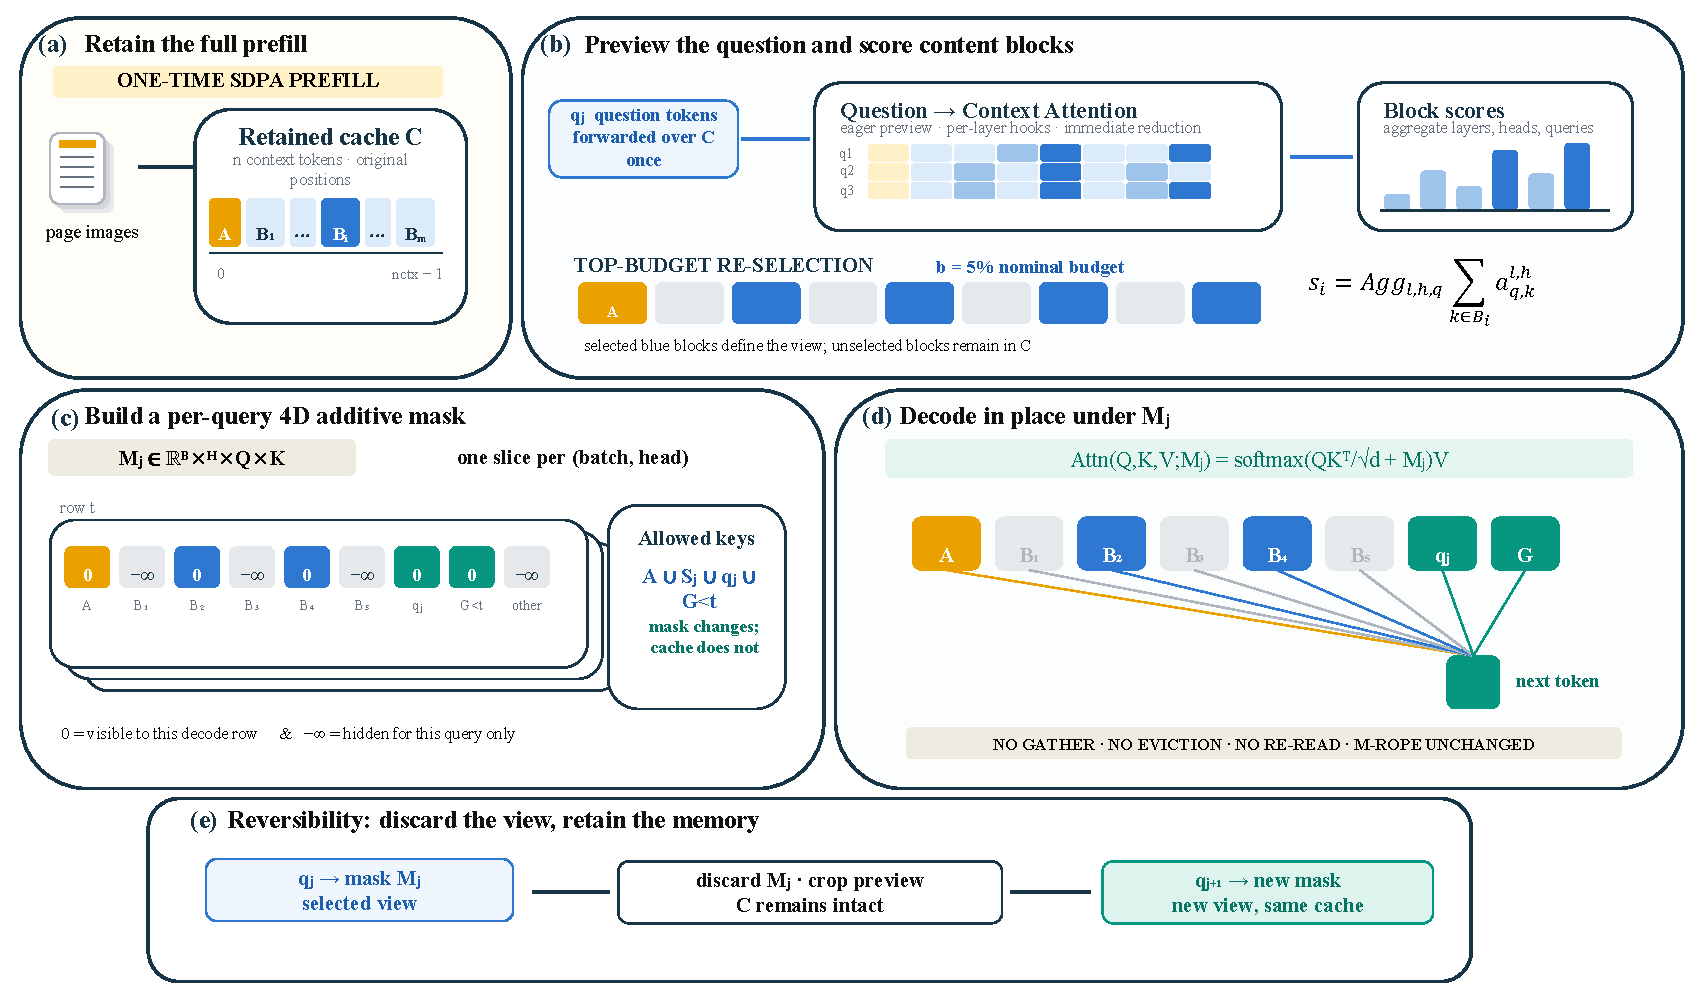
\includegraphics[width=0.92\textwidth]{figures/figure2_paq_kv_detailed_v1_editable.pdf}
\caption{
Detailed PAQ-KV restricted-attention mechanism.
\textbf{A:} The frozen reader prefills the document once and retains the full KV cache \(C\), including the always-keep scaffold \(\mathcal{A}\) and page-aligned 64-token blocks \(B_1,\ldots,B_m\), at their native M-RoPE positions.
\textbf{B:} For each question \(q_j\), an eager-attention preview captures question-to-context attention using per-layer hooks. Attention mass is aggregated into block scores, and the highest-scoring blocks \(S_j\) are retained under the nominal \(5\%\) decode-attention budget. The preview is then cropped so that questions cannot contaminate subsequent queries.
\textbf{C:} PAQ-KV constructs a query-specific additive mask \(M_j \in \mathbb{R}^{B \times H \times Q \times K}\), assigning \(0\) to \(\mathcal{A} \cup S_j \cup q_j \cup G_{<t}\) and \(-\infty\) to all other keys.
\textbf{D:} Decoding proceeds directly over the intact cache under \(M_j\), without gathering or evicting K/V, re-reading the document, or changing positional indices. After answering, \(M_j\) is discarded, and the same complete cache is re-masked for \(q_{j+1}\).
}\label{fig:paqkvmask}
\end{figure*}


\begin{figure*}
    \centering
    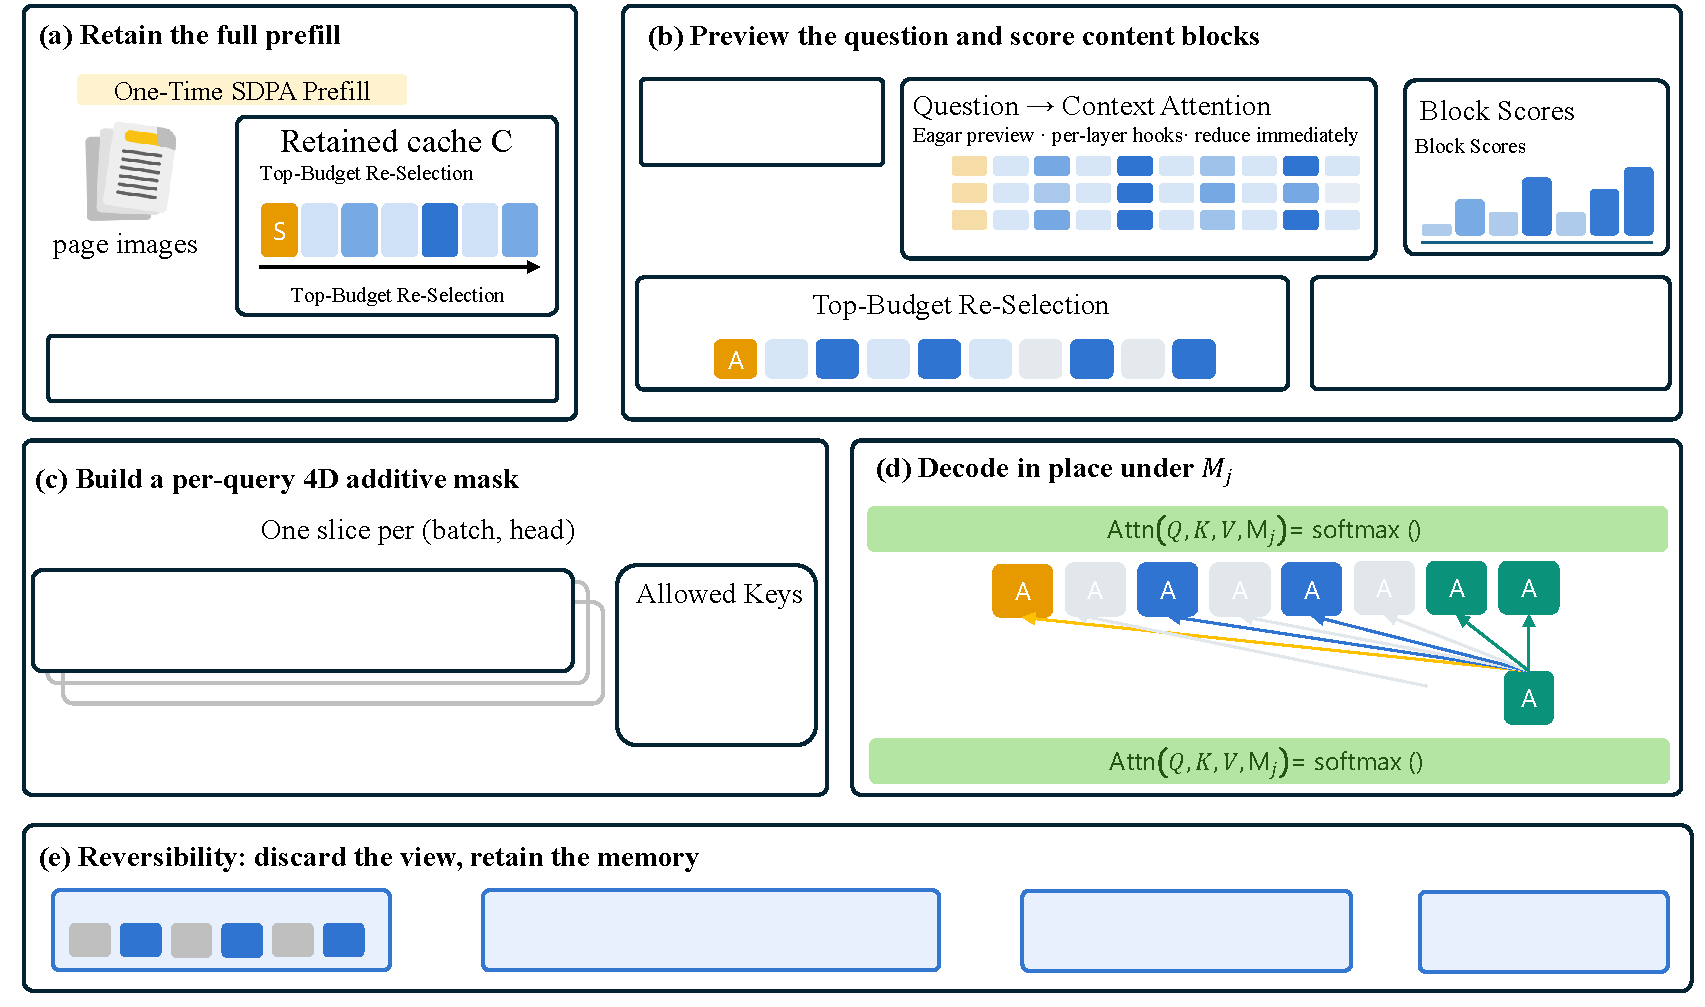
\includegraphics[width=0.95\linewidth]{figures/framework.pdf}
    % Artwork notes for the redraw: panel (e)'s in-figure title still reads
    % "discard the view, retain the memory" (view framing is banned; retitle in
    % reversibility terms), and panel (b) has the typo "Eagar preview".
    \caption{\paqc{} in five steps. \textbf{(a)} The document's page images are
    prefilled once with SDPA and the full KV cache $C$ is retained, scaffold
    $\mathcal{A}$ included. \textbf{(b)} Each question is previewed with eager
    attention and per-layer hooks; attention from the question tokens to the
    context is reduced to scores over 64-token page-aligned blocks, and the
    top blocks are re-selected under the budget. \textbf{(c)} The selection
    becomes a per-query four-dimensional additive mask, one slice per batch
    and head, whose allowed keys are the scaffold, the selected blocks, the
    question, and the generated tokens. \textbf{(d)} The answer is decoded in
    place under $M_j$ over the intact cache. \textbf{(e)} After answering, the
    mask is discarded and the complete cache remains, so the next question
    re-selects from the same memory: selection is reversible.}
    \label{fig:placeholder}
\end{figure*}

\subsection{Exactness and Reversibility}
A decode-identity audit, pre-registered as a kill criterion, checked the mask
path against the native decode on six document-query pairs spanning $32$K to
$122$K tokens: in all six cases an all-true mask produced zero mask-specific
argmax changes, so we claim identity in the audited cases, not in general
(Appendix~\ref{app:reversibility} gives the audit detail). Because nothing is
discarded, every selection is furthermore \emph{reversible}: the next query
re-scores and re-masks the same complete cache, whereas whatever commit-once
eviction dropped is unrecoverable. Reversibility is the axis our evaluation
isolates (\S\ref{sec:setup-stats}, \S\ref{sec:results-isolation}).

\paragraph{Relation to existing designs.} \paqc{} is not CAPS (a separate scoring VLM, per-page full re-forwards, page granularity, single-query); it is not coarse-to-fine page routing with a full-resolution re-read (\paq{}~v1, our own earlier page-level system, Appendix~\ref{app:pagelevel}); and it is not eviction (the mask is per-query and reversible). The mask route is the \emph{accuracy} path; physically gathering the cache for savings is a separate efficiency claim, and one we do not make here.

\section{Experimental Setup}\label{sec:setup}

\subsection{Benchmarks, Pins, Reader}
We evaluate on LongDocURL \citep{deng2025longdocurl} and MMLongBench-Doc
\citep{ma2024mmlongbench}, both as page images, and add two development-grade
cells built from MMDocRAG \citep{dong2025mmdocrag} and MMDocIR
\citep{dong2025mmdocir} (\S\ref{sec:results-scope}). Each cell uses a fixed,
seed-frozen evaluation subset (a \emph{pin}): the confirmatory pin holds 80
documents per cell, with 463/440 complete queries and 5.79/5.50 gold-bearing
queries per document (LongDocURL/MMLongBench-Doc), each document prefilled
once at a nominal ${\approx}64$K-token context so every query's evidence is
present in one prefill; Appendix~\ref{app:method-materials} gives the
construction rules. A 30-document screen pin is its strict prefix, and
results are additionally checked on the 50 new documents only
(\S\ref{sec:results-isolation}). The reader is Qwen3-VL-8B
\citep{qwen3vl2025}, frozen throughout: scaled dot-product attention serves
prefill and reading, and eager attention is enabled only during the per-query
preview so question-to-content attention can be captured. Page-level arms
operate at a matched page budget $b \in \{2.5\%, 5\%, 10\%\}$, with the
pre-registered gate budget at $b=5\%$; accuracy is the benchmark's
document-VQA scorer. The primary results are a Qwen3-VL-8B case study;
\S\ref{sec:results-crossreader} ports the full method to three further
readers as a development-pin generality control.

\paragraph{Evidence status.} Primary accuracy results use the
80-document-per-cell development pins unless labelled otherwise; mechanism,
budget, and integrity analyses use smaller screening subsets whose sizes are
stated where used. \emph{Sealed} here means a disjoint held-out test set
evaluated exactly once under a frozen protocol: only the MMLongBench-Doc
\paqc{}-versus-ColQwen2 comparison was sealed-evaluated, on a fresh
45-document cell (\S\ref{sec:results-mmlo}); the sealed LongDocURL documents
remain unevaluated. The cross-reader results, the MMDocRAG and MMDocIR-QA
cells, the same-cohort baseline panels, and the MMDocIR selection-quality
analysis are development-grade additions with single runs and no pre-frozen
bars (\S\ref{sec:results-scope}; Appendices~\ref{app:xrb}
and~\ref{app:mmdocir}).

\subsection{Statistical Protocol}\label{sec:setup-stats}
All inference uses a document-cluster paired bootstrap: queries of one
document share the document and (for stale arms) the single committed subset,
so bootstrapping over queries would be anti-conservative pseudoreplication.
Intervals resample documents with replacement within each cell (10{,}000
draws, seed 0). Paired contrasts are reported as the mean difference $\Delta$
with its two-sided 95\% confidence interval (CI), written $\Delta$ $[l, u]$;
bare bracketed pairs after an effect denote this interval throughout. Every
pre-registered gate in this study is a criterion on the interval's lower
bound: a gate passes when the lower bound exceeds zero, or the stated margin,
and where that bound alone carries the argument we name it in words. Per-cell
results are primary; pooled contrasts use equal cell weighting and are
labelled. Every gate was frozen before its run.

\paragraph{The isolation gate.} That query-aware selection outperforms
query-agnostic eviction is both a known text result \citep{tang2024quest} and
a potential strawman. We therefore fix the tested axis to \emph{reversibility}:
every baseline runs its canonical scorer but is deployed stale, committed once
per document (query-aware scorers commit a min-max-normalized aggregate over
the document's first $M=\min(3,k)$ queries), while the fresh arm re-selects
per query. Reversibility is credited only if the fresh arm outperforms two
comparators. The first is its \emph{own} scorer committed once: scorer and
budget are identical, so the delta isolates the mechanism. The second is a
strong \emph{gold-informed} static subset, the top pages by gold-page
frequency across the document's queries: not deployable, and not provably
optimal, but immune to the weak-static artifact that invalidated an earlier
one-comparator gate. The gate is executed with \paqc{} itself as the fresh
arm at its native below-page granularity (the committed aggregate and the
gold-frequency scores are applied over the same 64-token blocks), on the full
80-document pins of both cells, post-fix code only; the bar, arms, budget,
seed, imputation policy, and code hashes were frozen and committed before the
run (Appendix~\ref{app:repro}).

\subsection{Baselines}
The executed panel (Appendix~\ref{app:panel}) compares, per query at matched
budget on the same pinned data and reader: ColQwen2 \citep{faysse2025colpali}
fresh and stale, CLIP \citep{radford2021clip} fresh, SnapKV fresh and stale,
the isolation arms above, random and truncation controls, and a query-blind
eviction family (H2O, a context-only FastV proxy, LOOK-M, and a KVzip
\texttt{recv\_max} proxy). The eviction arms are disclosed proxies that sit at
or below random page recall on these cells, so the trained retriever is the
binding comparison; we rest no claim on outperforming proxy eviction.
Full-context and gold-page-oracle rows are references, not competitors. The
training-free arm family is executed at matched page-set semantics on the
development reader for every cell of Table~\ref{tab:paqkv} and on all three
second readers (Appendix~\ref{app:xrb}).

\subsection{Methods Integrity}\label{sec:integrity}
Two independent code reviews caught defects that we repaired and quantified
rather than assumed away; Appendix~\ref{app:integrity} gives both accounts in
full. First, the per-query scoring loop reused the document prefill without
restoring it, so early queries contaminated later previews. The fix, cropping
the cache after every preview, is applied everywhere; every gate and headline
number postdates it, the confirmatory isolation gate was re-executed in full
on post-fix code with runtime verification, and the key isolation contrast is
essentially unchanged ($+0.264$ clean versus $+0.284$ polluted on a
24-document re-run). Second, the cached ColQwen2 baseline had loaded with its
trained final retrieval-projection LoRA silently zeroed. We patched the
loader, added a post-load assertion, and re-scored the comparator: the
correction is immaterial, with the MMLongBench-Doc improvement at $+0.077$
against both loaders and the LongDocURL contrast at $+0.019$ against both.
The corrected loader is used everywhere except the historical page-level
panel of Appendix~\ref{app:panel}, which also predates the cache fix
(${\approx}0.04$ absolute inflation) and is labelled as historical; no claim
rests on its absolute levels.

Separately, the study adopted a sealed-test discipline: the 80-document pin
is development-only, and a fresh, disjoint 45-document / 244-query
MMLongBench-Doc set was reserved and evaluated \emph{exactly once} under a
frozen, hash-guarded harness (Appendix~\ref{app:repro}). That one sealed
evaluation confirms the improvement out-of-sample (\S\ref{sec:results-mmlo});
the sealed LongDocURL documents were not evaluated.

\section{Results}\label{sec:results}

\subsection{Does Per-Query Re-Selection Matter?}\label{sec:results-isolation}

% Figure source: scripts/make_fig_forest_contrasts.py (values transcribed from
% isogate_macros / tab:contrasts / tab:crossreader verdict-backed numbers).
\begin{figure}[t]
\centering
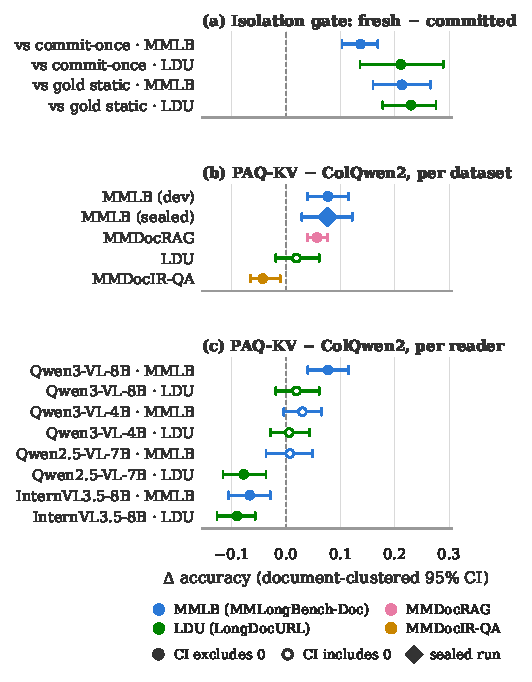
\includegraphics[width=\columnwidth]{figures/fig_forest_contrasts.pdf}
\caption{Key paired contrasts (mean $\Delta$ accuracy, document-clustered
bootstrap 95\% CIs). Color indexes the benchmark in every panel: blue
MMLongBench-Doc (MMLB), green LongDocURL (LDU), magenta MMDocRAG, yellow
MMDocIR-QA. Filled markers mark intervals excluding zero, open markers
intervals that include it; the diamond is the single sealed evaluation.
\textbf{(a)} The confirmatory isolation gate: \paqc{} minus its own scorer
committed once and minus a gold-informed static subset
(\S\ref{sec:results-isolation}). \textbf{(b)} \paqc{} minus ColQwen2-fresh
per dataset on Qwen3-VL-8B (\S\ref{sec:results-mmlo},
\S\ref{sec:results-scope}). \textbf{(c)} The same contrast per reader on the
development pins (\S\ref{sec:results-crossreader}). Exact values in
Appendix~\ref{app:contrasts} and~\ref{app:crossreader-table}.}
\label{fig:forest}
\end{figure}

The isolation gate runs at $b=5\%$ on all \isoKVNComplete{} pinned queries of
the confirmatory pin (80 documents per cell; zero skips), pitting \paqc{}
itself, per-query below-page re-selection over the retained cache, against
two comparators built from the same 64-token block scores. \paqc{} scores
$\isoKVLduFresh$/$\isoKVMmFresh$ (LongDocURL/MMLongBench-Doc), the identical
scorer committed once scores $\isoKVLduCommitAcc$/$\isoKVMmCommitAcc$, and
the gold-informed static scores $\isoKVLduStaticAcc$/$\isoKVMmStaticAcc$.
Both gate contrasts pass in both cells, by
$\isoKVLduCommitDelta$/$\isoKVMmCommitDelta$ over commit-once and
$\isoKVLduStaticDelta$/$\isoKVMmStaticDelta$ over the static
(Figure~\ref{fig:forest}a; full table in Appendix~\ref{app:isolation-table}).
The committed subset is not a strawman: it shares a third of the fresh arm's
blocks (mean Jaccard $0.368$) and still loses, and all three arms realize a
matched ${\approx}6.0\%$ of context. The contrast survives three robustness
checks (Appendix~\ref{app:reversibility}): re-running the statistics on only
the 50 documents outside the screen prefix ($+0.180$/$+0.206$ pooled), a
clean-cache page-level re-run ($+0.264$, lower bound $+0.187$), and a scorer
swap in which ColQwen2 itself collapses when committed once ($0.423$ fresh
versus $0.178$ stale), so reversibility is a property of the multi-query
regime rather than of our scorer. A pre-registered ``commitment-pressure''
mechanism gradient failed its formal interaction test and is retained as
exploratory only.

\subsection{Does \paqc{} Compete with Trained Retrieval?}\label{sec:results-mmlo}

% Contrast sources: paqc_topup_verdict.json / paqc_mmlo_topup_verdict.json /
% paq_colqwen_corrected_beat.json; sealed column: paq_sealed_final_sealed_verdict.json;
% MMDocRAG column: paq_mmdocrag_verdict.json (2026-07-25; development-grade);
% LongDocURL full/oracle contrasts: paqc_topup_fulloracle_posthoc.json (post-hoc,
% identical frozen instrument). Training-free baseline rows on LDU/MMLB:
% paq_verdict.json (page-level executed panel, Appendix app:panel).
% Realized-budget caption note + recall/stratification sentences in this section:
% research/paq_metrics_expansion.json (BASED afd8c7f).
\begin{table*}[t]
\centering\footnotesize
\setlength{\tabcolsep}{4pt}
\begin{tabular}{lcccc}
\toprule
 & LongDocURL & MMLongBench-Doc & MMDocRAG & MMDocIR-QA \\
 & \scriptsize 80 docs / 463 q & \scriptsize 80 docs / 444 q & \scriptsize 62 docs / 585 q & \scriptsize 80 docs / 538 q \\
\midrule
% LDU ColQwen2 cell: corrected loader as of 2026-07-26
% (research/paq_colqwen_corrected_beat_ldu.json: Jaccard 0.968, 25/463 re-read, immaterial per frozen rule).
% Same-cohort baseline rows (round 2): research/paq_xrb_verdict.json keys qwen3vl8b|{mmlongdoc,longdocurl};
% MMDocIR-QA column: research/paq_mmdocirqa_verdict.json; BM25/CAPS: paq_bm25*/paq_caps* verdicts.
% Round-3 fills (2026-07-26, commit b68b1c4): SnapKV-stale + CAPS on MMDocRAG/MMDocIR-QA,
% BM25 on MMDocIR-QA (benchmark ocr_text field, 99.5% coverage); 12-arm verdicts.
% CAPS MMLB = 0.3561 per paq_caps_verdict.json (generated/tab_main.tex shows 0.3567 -- flagged for reconciliation).
\paqc{}@5\% (\textbf{ours}) & \textbf{0.5315} & \textbf{0.4042}$^{*}$ & \textbf{0.4089}$^{*}$ & 0.3654 \\
ColQwen2-fresh (matched) & 0.5121 & 0.3282 & 0.3517 & \textbf{0.4080}$^{*}$ \\
\midrule
CAPS-style expert head (page) & 0.5182 & 0.3561 & 0.3667 & 0.3618 \\
BM25 (page retriever)$^\ddagger$ & 0.4030 & 0.2109 & 0.2793 & 0.3522 \\
SnapKV-fresh (page) & 0.4892 & 0.3243 & 0.1557 & 0.1987 \\
SnapKV-stale (commit-once) & 0.1873 & 0.0902 & 0.0750 & 0.1228 \\
CLIP-fresh & 0.1549 & 0.1624 & 0.1119 & 0.1400 \\
ColQwen2-stale (commit-once) & 0.2160 & 0.1365 & 0.1749 & 0.1583 \\
random & 0.0675 & 0.0218 & 0.0368 & 0.0807 \\
truncation & 0.0329 & 0.0410 & 0.0327 & 0.0876 \\
\midrule
full-context (ref.) & 0.5456 & 0.3965 & 0.4018 & 0.3785 \\
gold-page oracle (ref.; not strict) & 0.6092 & 0.4314 & 0.4028 & 0.4608 \\
\bottomrule
\end{tabular}
\caption{Main results: accuracy at the nominal 5\% budget per benchmark
(reader Qwen3-VL-8B). Bold marks the best non-reference arm per column;
$^{*}$ marks a paired \paqc{}-versus-ColQwen2 difference whose
document-clustered 95\% CI excludes zero (Appendix~\ref{app:contrasts}),
placed on the better arm. LongDocURL and MMLongBench-Doc are the 80-document
development pins; MMDocRAG and MMDocIR-QA are development-grade cells with
single runs and no pre-registered bars. The sealed MMLongBench-Doc
confirmation is deliberately not a column: it is shown in
Figure~\ref{fig:sealed} and Figure~\ref{fig:forest}b. All baseline rows share
\paqc{}'s post-fix frozen stack at matched page-set semantics.
$^\ddagger$BM25 text channels differ by corpus.
Appendix~\ref{app:table1-notes} gives realized budgets, text channels, and
cohort notes.}
\label{tab:paqkv}
\end{table*}

\paragraph{Main comparison.} On the 80-document development pin (444 queries
decoded; contrasts on the 440 with cached references), \paqc{}@5\% scores
$0.404$ versus $0.328$ for ColQwen2-fresh. The improvement of $+0.077$
(95\% CI $[+0.040,+0.115]$) meets the pre-registered per-cell bar with margin
(Figure~\ref{fig:forest}b; Table~\ref{tab:contrasts} in
Appendix~\ref{app:contrasts}). ColQwen2 here runs with its trained
retrieval-projection LoRA correctly applied; \S\ref{sec:integrity} documents
the loader defect we found and corrected and shows the correction is
immaterial to this comparison. Two development-pin re-slices sharpen where the
improvement comes from. At the same nominal budget the retriever delivers
\emph{more} gold evidence to the reader, not less: ColQwen2's kept pages cover
$0.539$ of gold-page tokens versus $0.344$ for \paqc{}'s selected blocks, yet
\paqc{} answers more accurately, so gold-evidence recall and answer accuracy
dissociate. And the paired improvement concentrates on cross-page evidence
($+0.109$ $[+0.052,+0.170]$, versus $+0.054$ $[+0.001,+0.108]$ on single-page
evidence), which directly supports the dispersed-evidence reading of this
cell. Appendix~\ref{app:anatomy} gives both recall notions and the full
evidence-type stratification.

% Figure source: BASED/research/paq_sealed_final_sealed_verdict.json via
% BASED/scripts/paq_fig_sealed_bar.py (nothing hand-entered).
\begin{figure}[t]
\centering
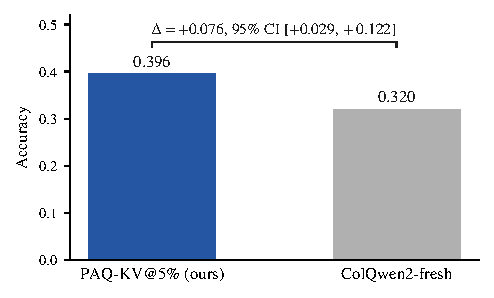
\includegraphics[width=0.92\columnwidth]{figures/fig_sealed_bar.pdf}
\caption{The sealed out-of-sample confirmation on MMLongBench-Doc: accuracy
of \paqc{}@5\% and ColQwen2-fresh on the fresh, disjoint 45-document,
244-query set, evaluated exactly once under the frozen harness
(\S\ref{sec:integrity}). The bracket reports the paired difference with its
document-clustered bootstrap 95\% CI; only this comparison was run on the
sealed set.}
\label{fig:sealed}
\end{figure}

\paragraph{Out-of-sample confirmation.} The improvement holds on the sealed
set (Figure~\ref{fig:sealed}). On 45 MMLongBench-Doc documents / 244 queries
with zero overlap with the development pin, under a harness whose bar,
comparator, budget, imputation policy, and code hashes were frozen before the
run (Appendix~\ref{app:repro}), \paqc{}@5\% scores $0.396$ versus
ColQwen2-fresh $0.320$: $+0.076$ (document-clustered 95\% CI
$[+0.029,+0.122]$), complete ($244/244$), unchanged under worst-case
missingness imputation, and closely matching the development estimate
($+0.077$). Only this comparison was sealed-evaluated; the reference arms are
development-pin only. This single evaluation is the strongest evidence in the
paper and directly addresses the development pin's reuse across the study.
On the development pin, \paqc{} at the same budget is indistinguishable from
full context ($+0.009$ $[-0.022,+0.040]$) and not statistically
distinguishable from the gold-page oracle ($-0.026$ $[-0.059,+0.008]$); the
latter interval permits material inferiority, so this is parity within noise
rather than demonstrated equality. A training-distribution audit found no
confirmed document-level overlap between the comparator's training mixture
and our corpora, and confirms it is trained for exactly this task family on
the same document genres (Appendix~\ref{app:repro}).

\paragraph{Mechanism checks.} On the 30-document screen the result survives
every mechanistic adversarial check: selection is query-dependent ($+0.329$
over random blocks), query-specific ($+0.698$ over wrong-question selection),
reversible ($+0.379$ over a first-query commit), and below-page granularity
helps over page level ($+0.054$ $[+0.011,+0.102]$).
Appendix~\ref{app:mechanism} details these screen analyses and their
caveats, including a screen-level budget-monotonicity failure that the
full-pin sweep of Appendix~\ref{app:budget-sweep} attributes to small-sample
noise.

\paragraph{Additional matched-budget baselines.} Table~\ref{tab:paqkv}
carries the full training-free family, re-run on \paqc{}'s own post-fix
cohort at matched page-set semantics. SnapKV-fresh, the strongest
training-free arm, scores pages from the same full-resolution prefill \paqc{}
uses and still trails it, by $+0.080$ $[+0.043,+0.119]$ on MMLongBench-Doc
and $+0.042$ $[-0.001,+0.092]$ on LongDocURL. A BM25 page retriever trails
\paqc{} by $+0.193$ and $+0.129$ $[+0.083,+0.176]$ respectively. The closest
chaser is a training-free \emph{page-level} CAPS-style expert-head control
with per-cell cross-validated head selection: \paqc{} exceeds it by $+0.048$
(95\% CI lower bound $+0.009$) on MMLongBench-Doc and is at parity on
LongDocURL, so the improvement over the trained retriever remains the
stronger claim. The full-pin budget sweep is in
Appendix~\ref{app:budget-sweep}; the query-blind eviction family remains in
Appendix~\ref{app:panel}, at or below random page selection. Two
pre-registered extensions of the scorer failed their pre-frozen gates and are
reported in Appendix~\ref{app:negatives}: a learned per-head attention
mixture did not transfer, and a single sharp expert head did not improve on
the diffuse block scorer.

\subsection{Where Does \paqc{} Help?}\label{sec:results-scope}

\paragraph{LongDocURL: a statistical tie.}\label{sec:results-longdocurl}
On the 80-document development pin (463 queries), \paqc{}@5\% posts a
positive point estimate over ColQwen2-fresh of $+0.019$ (95\% CI
$[-0.019,+0.061]$), which does not meet the pre-registered bar
(Figure~\ref{fig:forest}b). On this cell \paqc{} also sits below full
context, with an interval that includes zero, and clearly below the
gold-page oracle. The mechanism checks, query dependence and reversibility,
pass here too; what is missing is the margin. We treat this as a bounding
observation on where below-page selection helps rather than a second main
result, and defer the conversion-bound decomposition to
Appendix~\ref{app:limitations-detail}.

% Source: BASED/research/paq_mmdocrag_verdict.json (2026-07-25); rows in
% BASED/research/paq_mmdocrag_rows.jsonl (4680/4680, zero skips).
% Development-grade: single run, no pre-frozen bar, 62-document pin.
\paragraph{MMDocRAG: the improvement reproduces.}\label{sec:results-mmdocrag}
To test the dispersed-evidence reading beyond the two primary benchmarks, we
added MMDocRAG \citep{dong2025mmdocrag}, a retrieval-augmented document-QA
dataset with cross-modal, multi-page evidence chains (52\% of queries carry
cross-page evidence). MMDocRAG is corpus-adjacent to our pins, so a
document-name audit ran first: every document overlapping our development or
sealed pins was excluded before any experiment, leaving a fresh 62-document,
585-query development-grade cell (Appendix~\ref{app:repro} details the audit
and this pin's protocol deviations). The improvement over the trained
retriever reproduces: \paqc{}@5\% scores $0.409$ versus $0.352$, a margin of
$+0.057$ $[+0.040,+0.076]$ in the same class as the MMLongBench-Doc
development and sealed results. \paqc{} is again statistically
indistinguishable from its own full-context read and from the gold-page
oracle, and the oracle here barely exceeds full context, which is what
genuinely dispersed evidence predicts. The training-free baselines fall far
behind, committing either scorer once collapses it here too, and \paqc{}
clears even the benchmark-supervised expert-head control ($+0.042$
$[+0.030,+0.055]$; Table~\ref{tab:paqkv}). A query-cap check
(Appendix~\ref{app:repro}) confirms the capped cell did not manufacture the
result.

% Source: BASED/research/paq_mmdocirqa_verdict.json (2026-07-26; 80 docs /
% 538 q, 9 arms, zero skips). Development-grade: single run, no pre-frozen bar.
\paragraph{MMDocIR-QA: a retrieval-native reversal.}\label{sec:results-mmdocirqa}
MMDocIR's questions carry reference answers as well as gold evidence, so the
fresh-documents pin of Appendix~\ref{app:mmdocir} (80 documents, 538
queries, same overlap audit) also yields a fourth, development-grade QA cell,
the most retrieval-native of the four: its questions were written per
annotated layout for retrieval evaluation. Here the trained retriever wins.
ColQwen2-fresh scores $0.408$ versus $0.365$ for \paqc{}, a significant
deficit of $-0.043$ $[-0.065,-0.011]$, while \paqc{} remains
indistinguishable from its own full-context read and far above the
training-free arms (Table~\ref{tab:paqkv}). The cell rewards retrieval as
such: plain BM25 over the benchmark's own text ties \paqc{}, the supervised
expert-head control ties it as well, the trained retriever wins outright,
and, unlike the dispersed cells, the gold-page oracle sits well above full
context, so the cell's evidence regime, not selector quality, sets the sign.
Across the four cells the pattern is sharper than three positives would have
been: \paqc{} wins where evidence disperses (MMLongBench-Doc and MMDocRAG),
ties where conversion binds (LongDocURL), and loses where questions are
retrieval-native and evidence is concentrated (MMDocIR-QA);
Figure~\ref{fig:forest}b carries all five contrasts. This is the scope
condition of the conclusion, measured rather than asserted.

\paragraph{Cross-reader generality.}\label{sec:results-crossreader}
All results above use one reader. To test whether the effect is specific to
Qwen3-VL-8B, we ported the complete method (reader-own attention scoring,
block selection, masked decode) to three further VLMs: Qwen3-VL-4B (the same
architecture at half the parameters), Qwen2.5-VL-7B \citep{bai2025qwen25vl}
(the prior generation of the same family), and InternVL3.5-8B
\citep{wang2025internvl35} (a different VLM whose language backbone is
Qwen3). Every port passed the same all-true-mask decode-identity gate before
any accuracy number was read. The outcome is a gradient ordered by
architectural distance from the development reader
(Figure~\ref{fig:forest}c; full table and protocol in
Appendix~\ref{app:crossreader-table}). Qwen3-VL-4B largely preserves the
effect ($+0.030$ $[-0.004,+0.065]$ on MMLongBench-Doc) and, like the 8B,
scores above its own full context. Qwen2.5-VL-7B is a statistical tie
($+0.007$ $[-0.037,+0.049]$). InternVL3.5-8B falls significantly below both
its comparator ($-0.067$ $[-0.106,-0.029]$) and its own full context. On
LongDocURL every reader sits at or below its MMLongBench-Doc contrast with
the ordering preserved, consistent with that cell being conversion-bound. A
pre-registered development-only tuning study on InternVL found budget to be
the only effective lever: the deficit narrows monotonically to $-0.001$ at a
30\% budget, but the lower bound never clears zero, so the negative is not
an artifact of the 5\% budget or of the attention read-out
(Appendix~\ref{app:crossreader-table}).

The gradient tracks a measurable property: how well the host reader's own
attention retrieves evidence below page level. On the queries a reader
answers correctly from its own full context, its 5\% selection recovers
$0.88$ (Qwen3-VL-8B), $0.87$ (Qwen3-VL-4B), $0.70$ (Qwen2.5-VL-7B), and
$0.53$ (InternVL3.5-8B) of that accuracy. Since the effect survives halving
the reader within the same architecture but reverses across families, we
read the boundary as architectural rather than a matter of scale, and state
the scope condition plainly: \paqc{} is a white-box method whose benefit is
contingent on the host reader's attention being an effective below-page
retriever. \paqc{} nonetheless stays ahead of every training-free baseline
on every reader, including those where it loses to the trained retriever
(Appendix~\ref{app:xrb}). Three caveats attach: these are development-pin
generality controls, not sealed claims; the two non-Qwen3-VL readers run at
reduced realized context, so only within-reader contrasts are interpreted;
and InternVL3.5-8B's language backbone is Qwen3, so it is a cross-VLM test
but not a fully independent language architecture. Three further candidates
could not run the method under the pinned software stack and are reported as
incompatible rather than forced (Appendix~\ref{app:crossreader-table}).

\subsection{Systems Measurements}\label{sec:results-efficiency}
We measured the deployment profile of the true \paqc{} path (below-page
masked decode over the \emph{retained} full-document KV cache) against
ColQwen2-fresh and full context on an 8-document, 31-query systems subset of
the pin (single GPU, frozen configuration; Table~\ref{tab:systems}). \paqc{}
is roughly $2.25\times$ slower per online query than the retriever pipeline
and retains a multi-gigabyte per-document cache where the retriever stores a
megabyte-scale page index, but it is roughly $11\times$ faster than
re-reading the document for every question, and the one-time prefill
amortizes after about one query per document. \paqc{} therefore does not
reduce resident KV memory; it trades retained cache state for reversible
query-specific selection. The efficiency claim is simplicity and deployment
shape, not speed: no separately trained retriever checkpoint, no stored
vector index, one deployed model, and no repeated full-document prefills.

\begin{table}[t]
\centering\small
\setlength{\tabcolsep}{4pt}% permitted narrowing (AAAI kit)
\setlength{\tabcolsep}{1.2pt}%
\begin{tabular}{lcccccc}
\toprule
 & extra & per-doc & cold st. & online & amort. & VRAM \\
 & params & state & /doc (s) & /q (s) & /q (s) & (GiB) \\
\midrule
\paqc{} (ours)   & $0$        & $8.15$\,GiB & $11.3$ & $1.04$  & $3.07$  & $44.5$ \\
ColQwen2-fresh   & $2.246$\,B & $11$\,MiB   & $2.5$  & $0.46$  & $0.91$  & $21.8$ \\
full-context     & $0$        & n/a         & n/a    & $11.59$ & $11.59$ & $44.6$ \\
\bottomrule
\end{tabular}
\caption{Deployment profile on an 8-document / 31-query systems subset (frozen configuration, single GPU). ``Extra params'' = additional retriever/selector parameters beyond the shared reader. ``Cold start'' is the one-time per-document cost: full-document prefill for \paqc{}, page-embedding index build for ColQwen2. ``Amort.\ lat./q'' adds the cold start amortized at the development pin's observed $5.55$ queries/document to the online latency (at the systems subset's own $3.9$ queries/document the figures are $3.95$/$1.10$/$11.59$\,s). \paqc{}'s online latency decomposes into $0.19$\,s selection and $0.85$\,s masked decode; it is ${\approx}2.25\times$ slower and far heavier in resident state than ColQwen2, and ${\approx}11\times$ faster than full context (cold start amortized after $N{\approx}1.07$ queries/document). \paqc{}'s online latency excludes ${\approx}1.99$\,s/query of removable research-harness input reconstruction (component sum ${\approx}3.03$\,s/query in the current implementation); mean generated lengths differ across arms ($5.3$/$3.5$/$4.1$ tokens for \paqc{}/ColQwen2/full-context).}
\label{tab:systems}
\end{table}

\section{Conclusion}
\paqc{} turns a frozen VLM's own KV cache into a queryable, reversible
evidence store: prefill once, then per query re-select below-page blocks and
decode under a 4D restricted-attention mask over the intact cache, with no
gathering and M-RoPE preserved. Per-query re-selection beats committing the
identical scorer once in every tested cell, and the improvement over a
trained visual retriever at matched budget is confirmed on a sealed set
evaluated exactly once ($+0.076$, positive document-clustered lower bound).
Four datasets and four readers measure the scope: the advantage reproduces
where evidence is dispersed, ties where the cell is conversion-bound,
reverses where questions are retrieval-native, and requires a host reader
whose own attention is an effective below-page retriever. We offer that
scope law as the paper's hypothesis; a sealed-grade confirmation beyond
MMLongBench-Doc remains open.

\bibliography{references,references_extbench}

\appendix

% ============================================================================
% Appendix reorganized 2026-07-26 into four thematic sections (AAAI framing
% pass): A implementation/reproducibility, B complete results, C additional
% analyses, D limitations detail. All previous labels are preserved on the
% subsections; material moved out of the main body (integrity narratives,
% mechanism checks, negative results, cross-reader table, contrast table)
% lands here verbatim. This appendix will later become the separate
% supplementary document.
% ============================================================================

\section{Implementation and Reproducibility}\label{app:impl}

\subsection{Pin Construction, Algorithm, and Gate Materials}\label{app:method-materials}

\paragraph{Pin construction.} For each document we build the union of the
benchmark's own-document pages across that document's queries, dropping
cross-document 64K padding, so every query's evidence is present in one
prefill. Documents qualify with at least three gold-bearing queries and at
most 110 union pages, a bound that targets the nominal ${\approx}64$K-token
context at read resolution (realized lengths reach ${\approx}92$K on the
largest documents); selection is seed-0 frozen. Table~\ref{tab:pins}
summarizes the confirmatory pin.

\begin{algorithm}[t]
\caption{\paqc{}: per-query reversible below-page KV-block selection with a 4D restricted-attention mask}
\label{alg:paqc}
\begin{algorithmic}[1]
\REQUIRE document pages rendered as in the full-context arm ($\le$64K tokens); queries $q_1,\ldots,q_k$; nominal budget $b=5\%$; frozen VLM
\STATE prefill the document once; retain the full KV cache $C$ (context length $n_{\mathrm{ctx}}$); record page-aligned 64-token block spans $B_1,\ldots,B_m$ and the always-keep scaffold set $\mathcal{A}$
\FOR{each query $q_j$}
\STATE forward the tokenized question over $C$; capture question-to-context attention via per-layer hooks; \textbf{crop} $C$ back to $n_{\mathrm{ctx}}$
\STATE $\mathrm{score}(B_i) \gets$ aggregated question-row attention mass on block $B_i$'s positions
\STATE $S_j \gets$ top blocks by score at the nominal budget $b \cdot n_{\mathrm{ctx}}$
\STATE build the 4D additive mask $M_j$: decode rows may attend to $\mathcal{A} \cup S_j \cup q_j \cup{}$generated tokens; all other context positions get $-\infty$
\STATE decode the answer from $C$ under $M_j$; no gathering, so K/V positions and M-RoPE indices are unchanged
\STATE discard $M_j$; $C$ is intact for $q_{j+1}$
\ENDFOR
\end{algorithmic}
\end{algorithm}

\begin{table}[t]
\centering\small
\setlength{\tabcolsep}{4pt}% permitted narrowing (AAAI kit)
\begin{tabular}{lcc}
\toprule
 & LongDocURL & MMLongBench \\
\midrule
Documents & 80 & 80 \\
Complete queries at gate & 463 & 444 \\
Gold-bearing queries / doc & 5.79 & 5.50 \\
Median (mean) union pages & 44 (45.0) & 28 (36.5) \\
\bottomrule
\end{tabular}
\caption{The confirmatory evaluation pin. ``Complete queries'' are rows where every gated arm scored; the below-page gate completed all 907 pinned queries with zero skips, so no imputation was needed (the historical page-level run had 4 timeout-missing queries, immaterial under worst-case imputation).}
\label{tab:pins}
\end{table}

\subsection{Reproducibility and Protocol Notes}\label{app:repro}

\paragraph{Pre-registration discipline.} Every gate in this study was frozen (bars, comparators, budgets, imputation policy) before its run: the two-comparator isolation gate; the \paqt{} accuracy-evaluation bars (non-inferiority/improvement/inferior margins, per-cell power floors, adversarial missingness imputation); the per-head-mixture transfer gate; and the \paqc{} decode-identity kill criterion, screen gates, per-cell improvement bars, and sharp-scorer (V1) gate. Two early positives did not survive adversarial review and were retracted before this draft: a first isolation gate against the eviction family (invalidated by a weak-static artifact and replaced by the two-comparator gate), and an early ``outperforms the gold-page oracle'' claim (corrected to ``matches'' at power). The commitment-pressure mechanism hypothesis failed its formal test and is reported as exploratory.

\paragraph{Instrumentation.} All significance statements use one instrument: the document-cluster paired bootstrap (10{,}000 draws, seed 0, percentile intervals; equal-cell pooling), unit-tested alongside the gate and pairing logic. Evaluation pins are sha-256 checksummed and byte-verified before use; the screen pin is a strict prefix of the confirmatory pin, and independent-extension analyses use the 50 new documents per cell only. Figures are generated from the verdict artifacts by a single script; nothing is hand-entered. Per-query, per-arm rows, frozen-bar metadata, verdict files, and the adversarial review trail are retained and will be released with the code. The descriptive re-slices in Appendix~\ref{app:anatomy}, the realized-budget figures, the amortized-latency column of Table~\ref{tab:systems}, and the budget sweep of Appendix~\ref{app:budget-sweep} are additional reuses of the development pin and carry no pre-frozen bars.

\paragraph{Sealed-test protocol.} The 80-document confirmatory pin has been reused across this study and is therefore development-only. The fresh sealed set (zero overlap with the pin; 45 MMLongBench-Doc documents / 244 queries, plus 73 LongDocURL documents left unevaluated as out of scope) was evaluated \emph{exactly once} under a guarded, frozen harness: the confirmatory bar (complete-case document-clustered CI lower bound $>0$, with an adversarial worst-case-imputation fallback binding only under any missingness), the corrected-loader comparator, the 5\% budget, the seed, and sha-256 hashes of all eight code components plus the sealed pin were frozen before the run; the harness refuses the sealed pin absent an explicit authorization flag and a typed confirmation, aborts on any component-hash mismatch, and runs a blind non-scoring preflight that can abort without consuming the test. The single run produced the strongest claim in this paper: \paqc{}@5\% $0.396$ vs.\ ColQwen2-fresh $0.320$, $+0.076$ with document-clustered 95\% CI $[+0.029,+0.122]$ ($244/244$ complete, zero skips, robust to adversarial imputation; \S\ref{sec:results-mmlo}). The verdict, per-query rows, and a provenance manifest (pin and component hashes, resolved model revisions) are retained and released with the code.

\paragraph{Extended-benchmark overlap audit.} The two added corpora are
corpus-adjacent to ours: MMDocIR was sourced from existing DocVQA collections
including MMLongBench-Doc, and MMDocRAG was built over the MMDocIR document
pool. A document-name audit against our pins found substantial overlap,
including, name for name, the entire sealed MMLongBench-Doc cell inside
MMDocIR's pool. Every document overlapping either the development or the
sealed pins was excluded from the new pins before any experiment ran, so the
sealed reserve remains untouched at the document level; only document names
were read from the sealed pin file, and the audit artifact is retained. The
MMDocRAG pin's protocol deviations are disclosed here: 62 qualifying
documents is below the study's 80-document floor; queries are capped at 12
per document by seed-0 sampling (585 of 1{,}160 kept), a cap the main pins
never needed; pages render at 144\,DPI, matching the existing pins' pixel
scale; gold pages are the union of page identifiers over each query's gold
quotes, with the 0-based convention verified by text-fragment matching on 32
of 32 probes; and answers are scored by the study's shared document-VQA
evaluator. Because 28 of the 62 documents hit the twelve-query cap, we also
decoded the 575 uncapped remainder queries on the same documents: the
\paqc{}-versus-ColQwen2 contrast is $+0.035$ $[+0.019,+0.060]$ on the
remainder and $+0.046$ $[+0.032,+0.064]$ pooled, so the capped cell did not
manufacture the result. The MMDocIR-QA cell reuses the MMDocIR
selection-quality pin and scores against the benchmark's reference answers
with the same shared evaluator. The extended cells reuse the study's frozen
primitives (prefill, preview, selection, decode, the corrected ColQwen2
loader, the shared scorer, and the document-cluster paired bootstrap) but
froze no bars, ran each cell once, and constructed the pins on the day of
the runs. Two follow-ups closed this audit trail. A sealed-style MMDocRAG
reserve was investigated and is structurally empty: none of the 41 remaining
fresh documents qualify under the pin protocol (30 exceed the page ceiling,
11 lack three gold-bearing queries), so the MMDocIR-QA cell of
\S\ref{sec:results-mmdocirqa} serves as the independent corroboration lane
instead. And a training-distribution audit of ColQwen2, from its published
training mixture, found no confirmed document-level overlap with any of the
four evaluation corpora; MMDocIR's training split provably shares source
datasets with ColQwen2's mixture, but our cells draw only on its evaluation
pool, and web-crawled slices are unverifiable in both directions, so we
claim neither contamination nor proven disjointness.

\subsection{Methods-Integrity Detail}\label{app:integrity}

This section expands the summary of \S\ref{sec:integrity}.

\paragraph{Per-query cache pollution.} An independent code review found a
real bug in the per-query scoring loop used across this study: the runtime
mutates the retained cache in place, and the loop reused the document prefill
across a document's queries without restoring it, so query $q_i$ scored while
attending to $q_0\ldots q_{i-1}$. The fix, cropping the cache after every
per-query preview, is now applied everywhere, and its impact was quantified
rather than assumed. On a 24-document, 150-query clean-versus-polluted
re-run, the key isolation contrast is $+0.264$ clean versus $+0.284$
polluted, since the contrast largely cancels the bug when both arms share the
same scorer. Every gate and headline number in this paper postdates the fix,
including the confirmatory isolation gate of \S\ref{sec:results-isolation},
which was re-executed in full on post-fix code with \paqc{} as the fresh arm
and verified at runtime (cache-length assertions after every preview and
decode, plus an order-invariance probe per cell that recomputes a query's
preview after all other queries and requires bit-identity). The one
surviving pre-fix artifact is the historical page-level panel of
Appendix~\ref{app:panel}, whose absolute fresh-arm accuracy carries
${\approx}0.04$ inflation; it is labelled as historical and no claim rests
on its absolute levels. Appendix~\ref{app:reversibility} quantifies the
pollution mechanism itself.

\paragraph{Baseline-loader integrity.} A second independent review caught a
defect in the \emph{comparator}, not in our method: the cached ColQwen2
baseline had run with its trained final retrieval-projection LoRA
(\texttt{custom\_text\_proj}) silently zeroed. \texttt{vidore/colqwen2-v1.0}
is a PEFT adapter, and under our peft/transformers versions a key remap
inserted \texttt{language\_model} into the LoRA target path. The remap is
correct for the language-model layers but wrong for the top-level
\texttt{custom\_text\_proj}, so the checkpoint's projection-LoRA tensors
landed at a non-matching path and the final projection ran with base weights
only. Because the other adapter layers still loaded, the baseline stayed
functional and well above random, which masked the defect until we inspected
the load report and the projection weights directly. We patched the loader,
added a post-load assertion that the two \texttt{custom\_text\_proj} tensors
match the checkpoint, and re-scored ColQwen2. The correction is immaterial to
the main result. Fixed-versus-broken gold-page recall at the 5\% budget is
$0.539$ versus $0.534$. The top-5\% page selections overlap at Jaccard
$0.947$, with only $34$ of $444$ queries changing any selected page.
Re-reading those changed queries moves fresh-read accuracy by $-0.0002$
($0.3282$ corrected versus $0.3284$ broken), and the improvement over
ColQwen2 is $+0.077$ against both loaders (95\% CI lower bounds $+0.040$
corrected and $+0.039$ broken), so the main result is not loader-inflated.
The corrected loader is used for the main MMLongBench-Doc comparison
(development and sealed), the MMDocRAG cell, the systems measurement, and,
as of the same-protocol LongDocURL close-out, the LongDocURL comparison as
well (top-5\% selections overlap at Jaccard $0.968$; 25 of 463 queries
changed selection and were re-read; the comparator moves from $0.5124$ to
$0.5121$ and the contrast is $+0.019$ against both loaders, so the
correction is immaterial there too). Only the historical page-level panel
retains the earlier loader and is labelled as such.

\section{Complete Experimental Results}\label{app:results}

\subsection{Key Paired Contrasts}\label{app:contrasts}

Table~\ref{tab:contrasts} reports the paired contrasts summarized in
Figure~\ref{fig:forest}b.

\begin{table*}[t]
\centering\scriptsize
\setlength{\tabcolsep}{3pt}
\begin{tabular}{lcccc}
\toprule
 & \multicolumn{3}{c}{$\Delta$ (95\% CI), \paqc{} minus} & \\
\cmidrule(lr){2-4}
Benchmark & ColQwen2-fresh & full-context & gold-page oracle & Bar \\
\midrule
LongDocURL & $+0.019\,[-0.019,+0.061]$ & $-0.014\,[-0.031,+0.003]$ & $-0.078\,[-0.116,-0.040]$ & \textsc{not met} \\
MMLongBench-Doc & $+0.077\,[+0.040,+0.115]$ & $+0.009\,[-0.022,+0.040]$ & $-0.026\,[-0.059,+0.008]$ & \textbf{\textsc{met}} \\
MMLB (sealed) & $+0.076\,[+0.029,+0.122]$ & -- & -- & \textbf{\textsc{met}} \\
MMDocRAG & $+0.057\,[+0.040,+0.076]$ & $+0.007\,[-0.004,+0.018]$ & $+0.006\,[-0.009,+0.022]$ & none frozen \\
MMDocIR-QA & $-0.043\,[-0.065,-0.011]$ & $-0.013\,[-0.049,+0.012]$ & $-0.095\,[-0.158,-0.022]$ & none frozen \\
\bottomrule
\end{tabular}
\caption{Key paired contrasts for Table~\ref{tab:paqkv}: mean paired
difference $\Delta$ with its document-clustered bootstrap 95\% confidence
interval (10{,}000 draws; \S\ref{sec:setup-stats}). The pre-registered
per-cell bar (final column) passes when the CI lower bound of the
ColQwen2-fresh contrast exceeds zero; dashes denote arms not run on the
sealed set. On LongDocURL \paqc{} is below full context, with an interval
that includes zero, and below the gold-page oracle, with an interval that
excludes zero; on MMLongBench-Doc and MMDocRAG it is statistically
indistinguishable from both references. On MMDocIR-QA the trained retriever
significantly outperforms \paqc{}, which remains indistinguishable from its
own full-context read; \S\ref{sec:results-mmdocirqa} interprets the
four-cell pattern. The MMDocRAG and MMDocIR-QA cells are development-grade,
so no bars were frozen there.}
\label{tab:contrasts}
\end{table*}

\subsection{Notes on Table~\ref{tab:paqkv}}\label{app:table1-notes}

SnapKV-fresh scores pages from the same full-resolution prefill \paqc{}
uses, which roughly doubles it over the historical coarse-preview panel of
Appendix~\ref{app:panel}; we treat the same-cohort form as the fair one.
BM25 text channels differ by corpus: LongDocURL has no born-digital text
layer, so its cell uses a tesseract OCR channel (98.1\% of pages recovered),
the MMDocIR-QA cell uses the benchmark's own OCR text field (99.5\%
coverage), and the other cells use born-digital text. The LongDocURL
ColQwen2 cell uses the corrected loader (\S\ref{sec:integrity}).
MMLongBench-Doc decodes 444 queries; paired contrasts use the 440 with
cached references (the 4 \texttt{mi\_phone} rows lack cached references).
Realized budgets on MMLongBench-Doc: \paqc{} attends a mean $6.0\%$ of the
prefill context (median $6.0$, range $5.5$ to $7.5\%$), including the
always-attended non-visual prefix; ColQwen2 keeps whole pages, a mean
$4.6\%$ of pages under whole-page rounding.

\subsection{Confirmatory Isolation Gate Table}\label{app:isolation-table}

Table~\ref{tab:isolation} gives the full confirmatory isolation-gate values
behind \S\ref{sec:results-isolation} and Figure~\ref{fig:forest}a.

% Source: BASED/research/paq_isogate_kv_verdict.json via scripts/paq_isogate_tex.py
% (below-page gate, 2026-07-26; nothing hand-entered).
\begin{table*}[t]
\centering\small
% GENERATED by scripts/paq_isogate_tex.py 2026-07-26 01:33 — DO NOT EDIT BY HAND
% source: research/paq_isogate_kv_verdict.json (pin research/paq_confirm_pin.json sha 01f4e203ec67c2d5; n_complete=907/907; verdict=REVERSIBILITY_ISOLATED_BELOWPAGE)
\begin{tabular}{lccc}
\toprule
Contrast at $b{=}5\%$ & LongDocURL & MMLongBench-Doc & pooled (equal-cell, secondary) \\
\midrule
fresh $-$ same-scorer commit-once & $+0.211$ $[+0.136,+0.289]$ & $+0.137$ $[+0.103,+0.169]$ & $+0.174$ $[+0.132,+0.215]$ \\
fresh $-$ gold-informed static & $+0.230$ $[+0.178,+0.276]$ & $+0.213$ $[+0.160,+0.266]$ & $+0.221$ $[+0.184,+0.256]$ \\
\midrule
arm means (fresh / commit-once / static) & $0.531$ / $0.320$ / $0.301$ & $0.405$ / $0.268$ / $0.192$ & --- \\
\midrule
Verdict & \multicolumn{3}{c}{\textsc{reversibility isolated} (all $\lb > 0$, both cells)} \\
\bottomrule
\end{tabular}

\caption{Confirmatory below-page isolation at $b{=}5\%$ on all \isoKVNComplete{} pinned queries (accuracy; \paqc{} as the fresh arm; post-fix code; document-cluster paired bootstrap; contrast rows report $\Delta$ with 95\% CIs). The two-comparator bar was frozen and committed before the run; the per-cell contrasts are the pre-registered primary, the pooled column is secondary.}
\label{tab:isolation}
\end{table*}

\subsection{Cross-Reader Results in Full}\label{app:crossreader-table}

% Sources: internal companion note paq_cross_reader_generality.tex (tab:main,
% tab:longdocurl, tab:internvl-frontier; verdict JSONs + identity audits in
% BASED/research/ and research/reviews/paq_second_vlm_2026-07-22/). The
% Qwen3-VL-8B row repeats Table~\ref{tab:paqkv}'s verified values.
% Second-reader LongDocURL full-context (ref.) values = means.full_q25/full_iv
% from BASED/research/paq_{qwen3vl4b,qwen25vl,internvl}_longdocurl_verdict.json
% (decoded in the 2026-07-24 runs, 463/463 complete; means recomputed from the
% per-query results.jsonl on 2026-07-25, exact match).
\begin{table}[t]
\centering\scriptsize
\setlength{\tabcolsep}{2pt}% permitted narrowing (AAAI kit)
\begin{tabular}{lcc}
\toprule
Method & LDU & MMLB \\
\midrule
\multicolumn{3}{c}{Qwen3-VL-8B (development reader; ${\sim}69$K ctx)} \\
\midrule
\paqc{}@5\% (ours) & \textbf{0.5315} & \textbf{0.4042} \\
ColQwen2 (matched) & 0.5121 & 0.3282 \\
full-context (ref.) & 0.5456 & 0.3965 \\
$\Delta$ (95\% CI) & $+0.019\,[-0.019,+0.061]$ & $+0.077\,[+0.040,+0.115]$ \\
\midrule
\multicolumn{3}{c}{Qwen3-VL-4B (same architecture; ${\sim}69$K ctx)} \\
\midrule
\paqc{}@5\% (ours) & \textbf{0.4966} & \textbf{0.3640} \\
ColQwen2 (matched) & 0.4908 & 0.3336 \\
full-context (ref.) & 0.5024 & 0.3480 \\
$\Delta$ (95\% CI) & $+0.006\,[-0.028,+0.043]$ & $+0.030\,[-0.004,+0.065]$ \\
\midrule
\multicolumn{3}{c}{Qwen2.5-VL-7B (same family, prior gen.; ${\sim}52$K ctx)} \\
\midrule
\paqc{}@5\% (ours) & 0.3953 & \textbf{0.2698} \\
ColQwen2 (matched) & \textbf{0.4728} & 0.2623 \\
full-context (ref.) & 0.4558 & 0.3237 \\
$\Delta$ (95\% CI) & $-0.078\,[-0.116,-0.037]$ & $+0.007\,[-0.037,+0.049]$ \\
\midrule
\multicolumn{3}{c}{InternVL3.5-8B (cross-family, Qwen3 LM; ${\sim}36$K ctx)} \\
\midrule
\paqc{}@5\% (ours) & 0.2186 & 0.1876 \\
ColQwen2 (matched) & \textbf{0.3081} & \textbf{0.2542} \\
full-context (ref.) & 0.2961 & 0.2637 \\
$\Delta$ (95\% CI) & $-0.090\,[-0.127,-0.057]$ & $-0.067\,[-0.106,-0.029]$ \\
\bottomrule
\end{tabular}
\caption{Cross-reader generality at the 80-document development pins (LDU = LongDocURL, 463 queries; MMLB = MMLongBench-Doc, 444 queries). Within each reader block, \paqc{} (the reader's own attention selects ${\approx}5\%$ of blocks) is compared with the same reader reading the top-5\% pages ranked by the cached ColQwen2 scores, so every contrast is within-reader at matched budget; the reader's own full context is a reference, not a competitor. Bold marks the better of the two matched-budget arms per column by point estimate; significance is carried by the contrast rows, which report the \paqc{}-minus-ColQwen2 difference with its document-clustered 95\% CI. Block headers give the mean realized MMLongBench-Doc prefill length: the two non-Qwen3-VL readers run below the ${\approx}69$K budget because of their context ceilings, so only within-reader comparisons are interpreted. The Qwen3-VL-8B block repeats Table~\ref{tab:paqkv}; its MMLB improvement is additionally confirmed on the sealed set (\S\ref{sec:results-mmlo}). Qwen3-VL-4B reuses byte-identical input geometry (verified on all 80 documents), so that block is a pure size ablation.}
\label{tab:crossreader}
\end{table}

Table~\ref{tab:crossreader} gives the full cross-reader values behind
Figure~\ref{fig:forest}c. Every port had to pass the same all-true-mask
decode-identity gate (teacher-forced argmax parity against the native causal
decode, plus a restrictive mask that changes the output, on documents
spanning at least 30 pages) before any accuracy number was read. Against
their own full context on LongDocURL, Qwen3-VL-4B is indistinguishable
($-0.006$ $[-0.027,+0.017]$) while Qwen2.5-VL-7B and InternVL3.5-8B fall
short ($-0.060$ $[-0.100,-0.021]$ and $-0.077$ $[-0.109,-0.047]$);
InternVL3.5-8B is also below its own full context on MMLongBench-Doc
($-0.076$ $[-0.113,-0.041]$).

\paragraph{InternVL tuning study.} A pre-registered development-only tuning
study on InternVL3.5-8B (budgets $\{5,10,20,30\}\%$, four attention
read-outs, tuned on 40 documents and evaluated on the held-out 40) found
budget to be the only effective lever: the deficit narrows monotonically to
$-0.001$ at a 30\% budget, but the lower bound never clears zero at any
budget, and the tuned read-out adds nothing beyond budget ($+0.016$, 95\% CI
lower bound $-0.014$, paired against the default), so the negative is not an
artifact of the 5\% budget or of the default attention read-out.

\paragraph{Incompatible candidates.} Three further candidates (Molmo-7B-D,
MiniCPM-V-4.5, PaliGemma-2) could not run the method under the pinned
software stack (remote-code version drift for the first two; an
${\approx}8$K context that cannot hold a multi-page document for the third)
and are reported as incompatible rather than forced. This maps the method's
practical deployment envelope: a version-current implementation exposing
hookable attention and an honored 4D additive mask, and enough context to
prefill a whole document.

\subsection{Cross-Reader Baseline Panel}\label{app:xrb}

% Source: BASED/research/paq_xrb_verdict.json (per reader|cell) + cached port
% verdicts for the paqkv/colqwen/full reference rows. Development-grade.
The cross-reader results of \S\ref{sec:results-crossreader} compare \paqc{}
against ColQwen2-fresh and full context on the three second readers. This
appendix adds the remaining arm family at the same $b=5\%$ budget
(Table~\ref{tab:xrb}), with page-set semantics identical to the Qwen3-VL-8B
panel: the same cached CLIP and ColQwen2 page scores, the same commit-once
aggregation over the first $M{=}\min(3,k)$ queries, the same seed-0 random
and truncation controls, and the gold-page oracle read directly. The read
path is identical to each port's ColQwen2 comparator arm, so every number is
within-reader comparable. SnapKV arms are computed from each reader's
\emph{own} question-preview attention, aggregated to pages with the panel's
pooling, so SnapKV-fresh and SnapKV-stale are genuinely per-reader rather
than proxied from the development reader. All six reader-cell runs are
complete (907 queries by seven arms per reader, zero skipped rows), and
everything in this appendix is development-grade. The same arm family was
also executed on the development reader itself; those same-cohort values
replace the historical panel's baseline rows in Table~\ref{tab:paqkv}.

\begin{table}[t]
\centering\footnotesize
\setlength{\tabcolsep}{2.5pt}
% AUTO-GENERATED by BASED/scripts/paq_extended_tex_tables.py — do not edit by hand
\begin{tabular}{lcc}
\toprule
Arm & LDU & MMLB \\
\midrule
\multicolumn{3}{c}{Qwen3-VL-4B (same architecture)} \\
\midrule
\paqc{}@5\% (ours; cached) & 0.4966 & 0.3640 \\
ColQwen2-fresh (cached) & 0.4908 & 0.3336 \\
full-context (ref.; cached) & 0.5024 & 0.3480 \\
SnapKV-fresh & 0.4133 & 0.3034 \\
SnapKV-stale & 0.1332 & 0.0873 \\
CLIP-fresh & 0.1545 & 0.1805 \\
ColQwen2-stale & 0.2105 & 0.1576 \\
random & 0.0684 & 0.0296 \\
truncation & 0.0322 & 0.0423 \\
gold-page oracle (ref.) & 0.5839 & 0.4373 \\
\midrule
\multicolumn{3}{c}{Qwen2.5-VL-7B (same family, prior gen.)} \\
\midrule
\paqc{}@5\% (ours; cached) & 0.3953 & 0.2698 \\
ColQwen2-fresh (cached) & 0.4728 & 0.2623 \\
full-context (ref.; cached) & 0.4558 & 0.3237 \\
SnapKV-fresh & 0.2519 & 0.1265 \\
SnapKV-stale & 0.0574 & 0.0342 \\
CLIP-fresh & 0.1591 & 0.1354 \\
ColQwen2-stale & 0.2047 & 0.1245 \\
random & 0.0609 & 0.0253 \\
truncation & 0.0343 & 0.0394 \\
gold-page oracle (ref.) & 0.5380 & 0.3219 \\
\midrule
\multicolumn{3}{c}{InternVL3.5-8B (cross-family, Qwen3 LM)} \\
\midrule
\paqc{}@5\% (ours; cached) & 0.2186 & 0.1876 \\
ColQwen2-fresh (cached) & 0.3081 & 0.2542 \\
full-context (ref.; cached) & 0.2961 & 0.2637 \\
SnapKV-fresh & 0.0770 & 0.0889 \\
SnapKV-stale & 0.0537 & 0.0492 \\
CLIP-fresh & 0.1121 & 0.1498 \\
ColQwen2-stale & 0.1549 & 0.1068 \\
random & 0.0675 & 0.0377 \\
truncation & 0.0293 & 0.0385 \\
gold-page oracle (ref.) & 0.3408 & 0.3159 \\
\bottomrule
\end{tabular}

\caption{Baseline arm family on the three second readers at the 80-document
development pins (LDU = LongDocURL, MMLB = MMLongBench-Doc), $b=5\%$. The
\paqc{}, ColQwen2-fresh, and full-context rows are the cached values from the
cross-reader ports (identical to Table~\ref{tab:crossreader}); the remaining
arms are new runs with matched page-set semantics. Development-grade.}
\label{tab:xrb}
\end{table}

Three regularities stand out. First, \paqc{} stays ahead of every
training-free baseline on every reader, including the readers where it loses
to the trained retriever: SnapKV-fresh, the strongest such baseline, sits
significantly below \paqc{} in all six reader-cell combinations. Second,
SnapKV-fresh here is exactly the reader's own question-preview attention
selecting pages, so its absolute level reads out each reader's
attention-as-retriever quality; it falls across readers in the same order as
the recovery gradient of \S\ref{sec:results-crossreader}, so the selection
signal itself degrades in that order, independently of the block machinery.
Third, committing either scorer once collapses it on every reader, so the
multi-query staleness penalty is a property of the regime rather than of the
development reader. On InternVL3.5-8B the gold-page oracle additionally
exceeds the reader's own full-context accuracy, so that reader's bottleneck
is finding evidence rather than converting it: where the host's attention
retrieves poorly, a stronger selector recovers real accuracy that \paqc{}
leaves on the table.

Quantitatively: SnapKV-fresh sits below \paqc{} by $-0.061$
$[-0.096,-0.025]$ (MMLB) and $-0.083$ $[-0.144,-0.031]$ (LDU) on
Qwen3-VL-4B, by $-0.143$ on both Qwen2.5-VL-7B cells, and by $-0.099$ and
$-0.142$ on InternVL3.5-8B; its absolute level falls from $0.303$ to $0.127$
to $0.089$ across the three readers on MMLongBench-Doc, and from $0.413$ to
$0.252$ to $0.077$ on LongDocURL. On InternVL3.5-8B the gold-page oracle
exceeds full context by $+0.052$ $[+0.013,+0.094]$ on MMLB and $+0.045$
$[+0.007,+0.088]$ on LDU.

\subsection{Full-Pin Budget Sweep}\label{app:budget-sweep}
% Source: research/paq_budget_sweep_full_verdict.json (scripts/paq_budget_sweep_full.py,
% BASED 9b5114c): paqkv@{2.5,10}% decoded on the full 80-doc mmlongdoc pin (identity-gated
% against the cached frozen 5% selections; screen rows reused byte-identically) + matched
% corrected-loader ColQwen2 re-reads at each budget. Descriptive; bar frozen at 5% only.

\begin{table}[t]
\centering\small
\setlength{\tabcolsep}{2.5pt}%
\begin{tabular}{lccc}
\toprule
Budget & \paqc{} & ColQwen2@$b$ & $\Delta$ (95\% CI) \\
\midrule
$2.5\%$ & 0.389 & 0.291 & $+0.098\,[+0.058,+0.137]$ \\
$5\%$   & 0.404 & 0.328 & $+0.077\,[+0.040,+0.115]$ \\
$10\%$  & 0.405 & 0.370 & $+0.036\,[-0.001,+0.072]$ \\
\bottomrule
\end{tabular}
\caption{Full-pin budget sweep on MMLongBench-Doc (80 documents; matched budgets, corrected ColQwen2 loader). The $5\%$ row is the pre-registered main comparison (440 paired queries, Table~\ref{tab:paqkv}); the $2.5$/$10\%$ rows are descriptive (444 queries each; the pre-frozen bar was frozen at $5\%$ only). Realized fractions: \paqc{} $3.5$/$6.0$/$10.9\%$ of context, ColQwen2 $3.6$/$4.6$/$8.6\%$ of pages.}
\label{tab:budget-sweep}
\end{table}

The improvement is not a 5\%-only artifact, and on the full pin the earlier screen-only caveats resolve favorably. \paqc{}'s full-pin budget curve is monotone ($0.389$/$0.404$/$0.405$ at $2.5$/$5$/$10\%$), so the mild non-monotonicity previously observed on the 157-query screen subset ($0.397$/$0.404$/$0.398$) was small-sample noise. Against a ColQwen2 comparator re-read at the \emph{matched} page budget (Table~\ref{tab:budget-sweep}), \paqc{} is clearly ahead at $2.5\%$, ahead by the pre-registered margin at $5\%$, and ahead on point estimate at $10\%$ with an interval that just includes zero: the margin narrows as budget grows, because the retriever gains more from additional whole pages than \paqc{} gains from additional blocks. Against the fixed ColQwen2@$5\%$ comparator, every \paqc{} budget remains ahead ($+0.064$, $+0.077$, $+0.078$ at $2.5$/$5$/$10\%$, all lower bounds positive; 440 paired queries).

\subsection{Historical Page-Level Panel}\label{app:panel}
% RESOLVED 2026-07-26: this panel remains the HISTORICAL page-level cohort
% (pre-fix fresh arm, uncorrected ColQwen2 loader) and is labelled as such;
% the confirmatory isolation gate no longer rests on it (below-page gate,
% research/paq_isogate_kv_verdict.json). A same-cohort corrected-loader
% panel re-run remains optional future work (Priority 2 of the 07-26 rerun).

Table~\ref{tab:panel} reports every executed arm at the gate budget on the confirmatory pin. This is the historical page-level panel: its fresh arm predates the cache fix of \S\ref{sec:integrity} (${\approx}0.04$ absolute inflation) and its retrieval rows use the uncorrected ColQwen2 loader; it is retained as context for the arm family's ordering, and no headline claim rests on its absolute levels. The query-blind eviction family sits at or below random gold-page recall on these cells and is included for completeness (\S\ref{sec:setup}). Secondary pooled statistics: the fresh page-level selector exceeds the best arm of that family (SnapKV-stale) with min-over-family 95\% CI lower bound $+0.202$; fresh $-$ SnapKV-fresh $= +0.094$ $[+0.069,+0.122]$; fresh $-$ oracle $= -0.199$ $[-0.239,-0.161]$. Gold-page recall at $b{=}5\%$ (LongDocURL / MMLongBench-Doc): fresh page selector $0.494/0.443$; gold-informed static $0.381/0.373$; same-scorer commit-once $0.137/0.148$; ColQwen2-fresh $0.664/0.536$.

\begin{table}[t]
\centering\small
\setlength{\tabcolsep}{3.5pt}% permitted narrowing (AAAI kit)
\begin{tabular}{llcc}
\toprule
Group & Arm & LDU & MMLB \\
\midrule
\multirow{2}{*}{ours (page level)}
 & \paq{} (fresh) & \textbf{0.386} & \textbf{0.258} \\
 & attn\_max (alt-agg) & 0.337 & 0.152 \\
\midrule
\multirow{2}{*}{isolation}
 & same-scorer commit-once & 0.128 & 0.095 \\
 & gold-informed static & 0.278 & 0.154 \\
\midrule
\multirow{3}{*}{retrieval}
 & ColQwen2-fresh & 0.512 & 0.328 \\
 & ColQwen2-stale & 0.216 & 0.138 \\
 & CLIP-fresh & 0.155 & 0.164 \\
\midrule
\multirow{3}{*}{reference}
 & SnapKV-fresh & 0.298 & 0.157 \\
 & full-context & 0.546 & 0.397 \\
 & oracle-evidence & 0.609 & 0.431 \\
\midrule
\multirow{7}{*}{query-blind}
 & SnapKV-stale & 0.083 & 0.074 \\
 & H2O & 0.045 & 0.039 \\
 & FastV (proxy) & 0.045 & 0.031 \\
 & LOOK-M ($\to$H2O) & 0.045 & 0.039 \\
 & KVzip (proxy) & 0.047 & 0.048 \\
 & random & 0.068 & 0.022 \\
 & truncation & 0.033 & 0.041 \\
\bottomrule
\end{tabular}
\caption{Every executed arm, accuracy at $b{=}5\%$, per cell (LDU = LongDocURL, MMLB = MMLongBench-Doc), on the 903-query confirmatory panel (\texttt{paq\_verdict}). Query-aware arms marked fresh re-select per query; stale arms commit once per document. Cohort note: this 903-query confirmatory panel is the page-level study with the \emph{uncorrected} ColQwen2 loader (ColQwen2-fresh MMLB $0.328$); the below-page main comparison (Table~\ref{tab:paqkv}) is a distinct cohort (444 decoded / 440 paired) scored with the \emph{corrected} loader (ColQwen2-fresh MMLB $0.3282$, \S\ref{sec:integrity}). The loader correction is immaterial, so the shared reference rows agree to rounding.}
\label{tab:panel}
\end{table}

\subsection{MMDocIR: Below-Page Selection Quality}\label{app:mmdocir}

% Source: BASED/research/paq_mmdocir_selq_verdict.json. Development-grade.
MMDocIR \citep{dong2025mmdocir} provides expert gold at \emph{layout}
granularity: paragraphs, tables, figures, and charts as boxes on the page.
This is ground truth at exactly \paqc{}'s below-page granularity, which
neither QA benchmark offers. On a fresh-documents-only pin (80 documents, 538
queries, 641 gold layouts; the same exclusion audit as
Appendix~\ref{app:repro}), we score \paqc{}'s selected 64-token blocks
geometrically against the gold boxes: block token spans are mapped through
the reader's own patch grid to page-pixel rectangles, and we measure
gold-layout area coverage, layout hit rate, and gold-page recall at
$b\in\{5,10\}\%$ against random-block, truncation-block, and page-granularity
comparators at matched token budget (Table~\ref{tab:mmdocir}). No decoding is
involved, so the analysis isolates the selector from QA conversion entirely.
The same pin also yields the MMDocIR-QA accuracy cell of
\S\ref{sec:results-mmdocirqa}; there, the benchmark's reference answers skew
long, which depresses absolute levels under the study's short-answer scorer
without affecting the paired contrasts (a 30-probe scorer-fit check preceded
the run, and one query with an empty gold answer scores zero for all arms).

\begin{table}[t]
\centering\scriptsize
\setlength{\tabcolsep}{2pt}
% AUTO-GENERATED by BASED/scripts/paq_extended_tex_tables.py — do not edit by hand
\begin{tabular}{lcccc}
\toprule
Arm & layout cov. & layout hit & page recall & realized $b$ \\
\midrule
\multicolumn{5}{c}{nominal budget $b=0.05$} \\
\midrule
\paqc{} blocks (ours) & \textbf{0.689} & 0.834 & 0.903 & 5.3\% \\
page level (same scorer) & 0.693 & 0.694 & 0.694 & 7.7\% \\
random blocks & 0.056 & 0.141 & 0.449 & 5.3\% \\
truncation blocks & 0.079 & 0.087 & 0.095 & 5.4\% \\
\midrule
\multicolumn{5}{c}{nominal budget $b=0.1$} \\
\midrule
\paqc{} blocks (ours) & \textbf{0.778} & 0.895 & 0.960 & 10.3\% \\
page level (same scorer) & 0.791 & 0.792 & 0.792 & 12.2\% \\
random blocks & 0.114 & 0.273 & 0.720 & 10.2\% \\
truncation blocks & 0.125 & 0.127 & 0.138 & 10.3\% \\
\midrule
whole gold pages (upper ref.) & 1.000 & 1.000 & 1.000 & 5.6\% \\
\bottomrule
\end{tabular}

\caption{Selection quality against MMDocIR's sub-page gold layouts on the
80-document fresh pin (538 queries). ``Coverage'' is the fraction of
gold-layout area covered by selected blocks on gold pages; ``hit'' the
fraction of gold layouts touched at all; ``gold-page recall'' the fraction of
gold pages receiving any block. Development-grade.}
\label{tab:mmdocir}
\end{table}

Three observations. The selector finds sub-page evidence: at a realized
$5.3\%$ of context, \paqc{}'s blocks cover $0.689$ of gold-layout area, where
random blocks at the same budget cover $0.056$. This is the study's first
conversion-free measurement of the selection signal against human-annotated
sub-page ground truth. Below-page granularity buys reach rather than raw
area: the page-granularity arm, using identical attention scores aggregated
to pages, covers the same gold area but needs a realized $7.7\%$ of context
to do it under whole-page rounding, and at that higher spend still touches
fewer distinct gold layouts ($+0.140$ $[+0.097,+0.170]$ in \paqc{}'s favor)
and fewer gold pages. Blocks spread the same budget across more of the
question's evidence, which is the behavior the cross-page QA advantage of
Appendix~\ref{app:anatomy} suggested, now measured geometrically. Finally,
selecting every gold page in full would cost a realized $5.6\%$ of context on
this pin, essentially \paqc{}'s own spend, so a perfect page-level selector
could reach full coverage at matched budget; \paqc{} recovers $69\%$ of that
area with no supervision, from the reader's own attention, and the remaining
gap is the selection headroom that the oracle contrasts of
Appendix~\ref{app:xrb} price in accuracy terms.

\section{Additional Analyses}\label{app:analyses}

\subsection{Mechanism Checks in Detail}\label{app:mechanism}

On the 30-document screen (distinct from the 80-document confirmatory
cohort), the MMLongBench-Doc result survives every mechanistic adversarial
check: it is query-dependent (\paqc{} $-$ random-block selection $= +0.329$
$[+0.238,+0.418]$), query-specific (\paqc{} $-$ wrong-question selection $=
+0.698$ $[+0.603,+0.784]$, where the collapse supports query-specificity),
reversible (\paqc{} $-$ commit-once $= +0.379$ $[+0.273,+0.480]$; this
screen control commits the \emph{first query's} selection, a weaker
committed arm than the confirmatory gate's first-three-query aggregate,
which is why its margin exceeds the confirmatory $\isoKVMmCommitDelta$), and
below-page granularity helps over page level ($+0.054$ $[+0.011,+0.102]$).
These are development-pin screen analyses with disclosed caveats: the screen
budget-curve monotonicity gate failed on this cell ($0.398$ at 10\% vs.\
$0.402$ at 5\% on the 157-query screen subset), though the subsequent
full-pin sweep is monotone and attributes that failure to small-sample noise
(Appendix~\ref{app:budget-sweep}), and the effect they dissect is separately
confirmed out-of-sample on the sealed set (\S\ref{sec:results-mmlo}).

\subsection{Additional Reversibility Detail}\label{app:reversibility}
% Figure sources: BASED/research/paq_isogate_kv_verdict.json (leading four contrasts);
%                 BASED/research/paq_verdict.json; BASED/research/paq_revcrop_verdict.json;
%                 BASED/research/paqc_mmlongdoc_audit_verdict.json

\begin{figure*}[t]
\centering
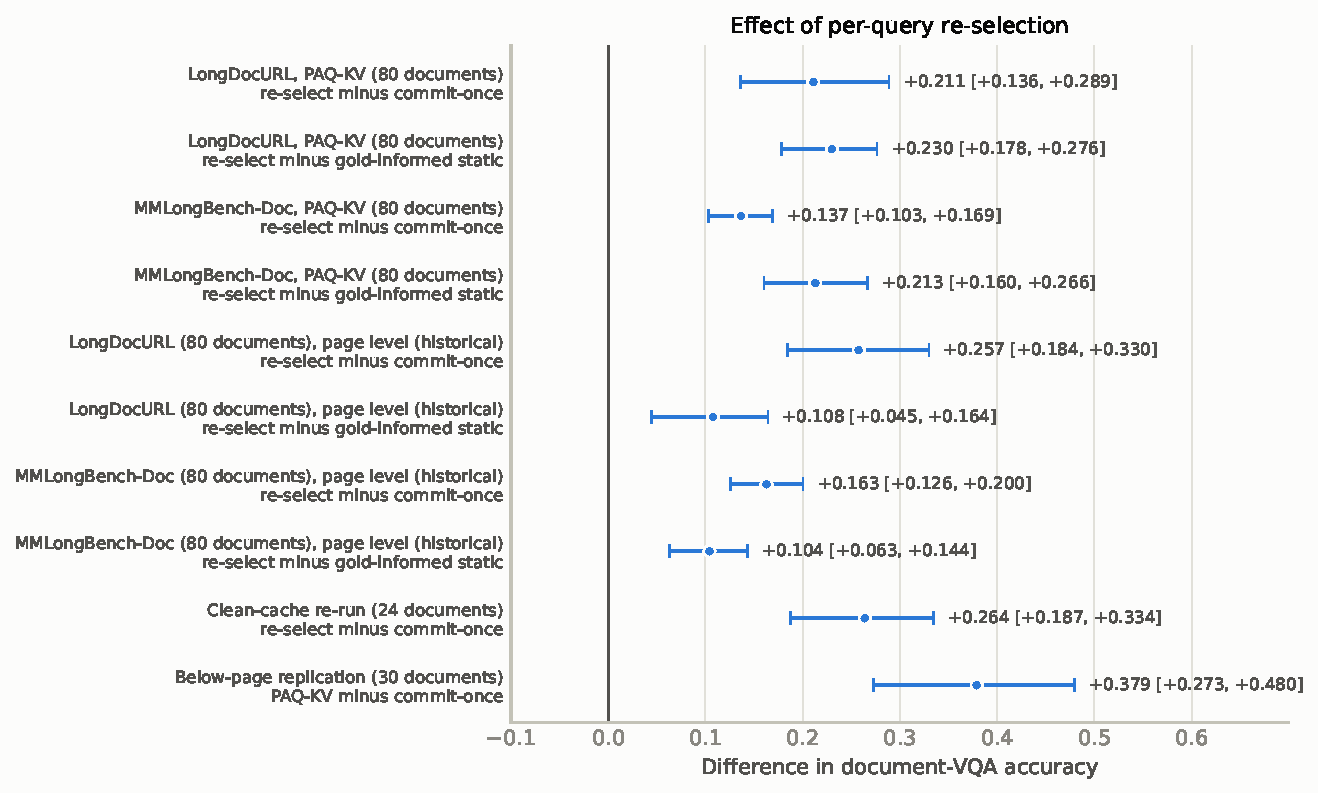
\includegraphics[width=0.7\textwidth]{fig_j_reversibility_light.pdf}
\caption{Document-clustered two-sided 95\% intervals for every executed isolation contrast. The leading four rows are the confirmatory below-page gate (\paqc{} as the fresh arm, full 80-document pins, post-fix code); below them, the historical page-level gate, the clean-cache re-run, and the 30-document below-page replication. Positive differences favor per-query re-selection; every interval excludes zero.}
\label{fig:reversibility}
\end{figure*}

\paragraph{Decode-identity audit detail.} The six audited document-query
pairs of \S\ref{sec:method} span $32$K to $122$K tokens, a stress range
deliberately wider than the evaluation pin. An earlier single greedy-token
divergence traced to the generation loop's mask-independent fast-path
kernel, not to the mask.

\paragraph{Robustness checks behind \S\ref{sec:results-isolation}.} First,
an independent extension: because the screen pin is embedded in the
confirmatory pin, we re-ran the statistics on the 50 new documents per cell
only ($n=586$ queries), where fresh over commit-once is $+0.180$
$[+0.124,+0.237]$ and fresh over the static $+0.206$ $[+0.161,+0.249]$
(pooled, equal-cell). Second, granularity and history: the same
two-comparator gate passed at page level on this pin (its pre-fix historical
run: $+0.257$/$+0.163$ over commit-once), and the page-level contrast
survives the clean-cache re-run of Appendix~\ref{app:integrity} ($+0.264$,
95\% CI lower bound $+0.187$), so the effect is not specific to block
granularity or to the fix. Third, scorer generality: the same
fresh-over-stale collapse holds for a retrieval scorer, with ColQwen2 fresh
at $0.423$ versus stale at $0.178$ (historical page-level cohort;
query-micro; equal-cell pooling agrees). The pre-registered
``commitment-pressure'' gradient failed its formal interaction test with
both intervals including zero.

Figure~\ref{fig:reversibility} summarizes the confirmatory below-page gate and its supporting replications. For the confirmatory gate, missingness is a non-issue: all 907 pinned queries completed with zero skips, so the pre-registered adversarial imputation guard (fresh scored $0$, comparators scored $1$ on any incomplete query) never binds. All three arms realize a matched ${\approx}6.0\%$ of context. Supporting analyses from the historical page-level run (pre-fix cohort, labelled): (i) \emph{answerable subset} (secondary, since it conditions on a model outcome): on queries where oracle-evidence scores exactly 1 ($n=407$), fresh $0.583$ vs.\ commit-once $0.182$ ($+0.395$ $[+0.324,+0.460]$) and vs.\ the static $0.382$ ($+0.204$ $[+0.135,+0.266]$); (ii) \emph{budget curves}: the fresh page-level selector dominates both static comparators at every budget in $\{2.5, 5, 10\}\%$ on both cells.

\paragraph{Cache-pollution quantification.} The in-place cache bug of \S\ref{sec:integrity} was quantified before being fixed: on a 6-documents-per-cell diagnostic (87 query-rows), the bug inflates gold-page recall by ${\approx}+0.05$ for a fixed scoring head and shifts selections (mean top-$B$ Jaccard clean vs.\ polluted $0.82$, drifting from $1.00$ at $q_0$ to $0.61$ at $q_6$), as expected for cumulative contamination. The recall gate behind the \paqt{} numbers was regenerated clean before any accuracy read (clean held-out expert recall $0.683$/$0.626$ vs.\ polluted $0.674$/$0.628$), and the clean cross-validation picks a more robust head. Absolute fresh-arm accuracy in the pre-fix confirmatory run carries ${\approx}0.04$ inflation (clean $-$ polluted $-0.041$ $[-0.077,-0.003]$ on the 24-document check); the isolation contrasts cancel the bug and stand.

\subsection{Selection Anatomy on MMLongBench-Doc}\label{app:anatomy}
% Source: BASED research/paq_metrics_expansion.json (scripts/paq_metrics_expansion.py,
% BASED commit afd8c7f): artifact-only re-slices of the retained 80-doc dev-pin rows;
% comparator = corrected ColQwen2 loader (cached rf + the 34 corrected re-read values);
% instrument = paq.cluster_lb95 (doc-cluster paired bootstrap, 10k draws, seed 0).

These are descriptive re-slices of the retained per-query development-pin rows (444 decoded / 440 paired, corrected ColQwen2 loader throughout); no pre-frozen bar attaches to them.

\paragraph{Gold-page recall vs.\ accuracy.} At the nominal 5\% budget, two recall notions bracket what each method hands the reader. Coverage-weighted (the fraction of gold-page \emph{tokens} the reader may attend; the budget-comparable notion, since ColQwen2 keeps whole pages): ColQwen2 $0.539$ vs.\ \paqc{} $0.344$, a deficit of $-0.195$ $[-0.236,-0.152]$ for \paqc{}. Any-block-touch (a gold page counts as recalled if any selected 64-token block overlaps it): \paqc{} $0.912$, but this notion flatters block granularity, since \paqc{}'s selections scatter over a median of $10$ pages per query. So the retriever delivers substantially more gold-evidence tokens at matched budget, touches fewer of the right pages, and still loses the accuracy comparison by $+0.077$ (Table~\ref{tab:paqkv}): recall-optimized selection is not accuracy-optimized selection, consistent with the sharp-scorer negative result (Appendix~\ref{app:negatives}).

\begin{table}[t]
\centering\small
\setlength{\tabcolsep}{1.3pt}%
\begin{tabular}{lrrccc}
\toprule
Stratum & $n$ & docs & \paqc{} & ColQ. & $\Delta$ (95\% CI) \\
\midrule
Chart       & 102 & 35 & 0.409 & 0.311 & $+0.098\,[+0.025,+0.176]$ \\
Figure      & 156 & 53 & 0.393 & 0.333 & $+0.060\,[-0.020,+0.143]$ \\
Layout      &  47 & 32 & 0.490 & 0.338 & $+0.152\,[+0.032,+0.252]$ \\
Pure text   & 144 & 52 & 0.356 & 0.308 & $+0.048\,[-0.010,+0.104]$ \\
Table       & 120 & 38 & 0.353 & 0.258 & $+0.096\,[+0.033,+0.163]$ \\
\midrule
Single-page & 256 & 74 & 0.526 & 0.471 & $+0.054\,[+0.001,+0.108]$ \\
Cross-page  & 184 & 70 & 0.238 & 0.129 & $+0.109\,[+0.052,+0.170]$ \\
\bottomrule
\end{tabular}
\caption{Paired \paqc{}@5\% $-$ ColQwen2-fresh (corrected loader) by MMLongBench-Doc evidence stratum on the 440-query paired cohort (document-cluster paired bootstrap). Evidence-source labels are the benchmark's own and are multi-label (a query counts under each listed source); single- vs.\ cross-page splits on the number of annotated gold pages. The improvement concentrates on cross-page evidence and on chart/table/layout sources; these are descriptive development-pin strata, not pre-registered claims.}
\label{tab:anatomy-strata}
\end{table}

\paragraph{Evidence-type stratification.} Table~\ref{tab:anatomy-strata} stratifies the main paired comparison by the benchmark's evidence annotations. The cross-page stratum roughly doubles the single-page contrast ($+0.109$ vs.\ $+0.054$), and the source strata whose intervals exclude zero (chart, table, layout) are those whose evidence a page-level retriever must fetch whole even when only a small region answers the question.

\subsection{Negative Results}\label{app:negatives}

\paragraph{Per-head mixture transfer gate.} No LoRA adapter was ever trained: this pre-frozen check failed first and stopped that line of work. We fit a logistic per-head mixture over all $36{\times}32=1{,}152$ (layer, head) question-to-page attention channels on off-benchmark provenance-checked data. The transfer gate fails: mixture gold-page recall is $0.652$/$0.594$ vs.\ $0.676$/$0.616$ for the single head, with pooled mixture $-$ single $=-0.023$ $[-0.037,-0.008]$ (907 queries), so the mixture overfits and this direction was closed. The best zero-benchmark-contact head (L21.H18) still coincides with the benchmark-supervised expert layer.

\paragraph{Sharp expert head as block scorer.} Replacing \paqc{}'s diffuse mean-attention block scorer (V0) with the sharp head L21.H18 (V1) fails the pre-frozen gate: on LongDocURL it only nudges the point estimate (from $0.5315$ to $0.536$; V1 $-$ ColQwen2 $= +0.024$ $[-0.012,+0.066]$) and does not separate from V0 (the V1$-$V0 95\% CI lower bound is $-0.011$, n.s.), while on MMLongBench-Doc it hurts (from $0.402$ to $0.381$ on the screen documents). As elsewhere in this study, recall-optimized selection is not accuracy-optimized selection.

\subsection{The Page-Level System in Detail}\label{app:pagelevel}
% RESOLVED 2026-07-26: predecessor material, retained as historical context.
% The confirmatory isolation evidence now comes from the below-page gate
% (\S sec:results-isolation / tab:isolation); this section documents the v1
% page router and its (pre-fix, uncorrected-loader) cohort, labelled as such.

The name \paq{} abbreviates ``Prefill once, Ask many Queries''; unsuffixed \paq{} denotes the earlier page-level router (v1) detailed in this appendix, \paqt{} its expert-head variant, and \paqc{} the below-page KV-mask method of the main text. All numbers in this section are on the 903-query confirmatory cohort (page-level arms), where ColQwen2-fresh scores $0.512$/$0.328$ (LDU/MMLB) with the uncorrected loader; it is distinct from the below-page cohort used in the main comparison (where the corrected-loader ColQwen2-fresh MMLB is $0.3282$, \S\ref{sec:integrity}). The loader correction is immaterial (\S\ref{sec:integrity}), so the page-level parity conclusions are unaffected.

\paragraph{The page router (\paq{} v1).} Pages are rendered at coarse resolution (${\approx}3.5$K visual tokens total, i.e.\ ${\approx}70$ tokens/page on a 50-page document) and prefilled once; per query, the question rows' attention (mean over heads, layers, and question tokens) scores pages; the top pages at budget $b$ are re-rendered at full resolution and read. This is page routing rather than KV compression, and it claims no memory savings.

\paragraph{Comparison against trained retrieval.} At $b=5\%$, ColQwen2-fresh scores $0.512$/$0.328$ vs.\ \paq{} $0.386$/$0.258$: pooled $-0.099$ $[-0.129,-0.072]$, a loss of roughly 10 points that holds on every stratum we examined (Figure~\ref{fig:retrieval}). Gold-page recall is consistent with a coverage contribution: ColQwen2-fresh $0.664$/$0.536$ vs.\ \paq{} $0.494$/$0.443$. Both scorers collapse when committed once (ColQwen2 stale $0.216$/$0.138$), reproducing the reversibility pattern with a second scorer family.

% Figure source: BASED/research/paq_verdict.json
\begin{figure}[t]
\centering
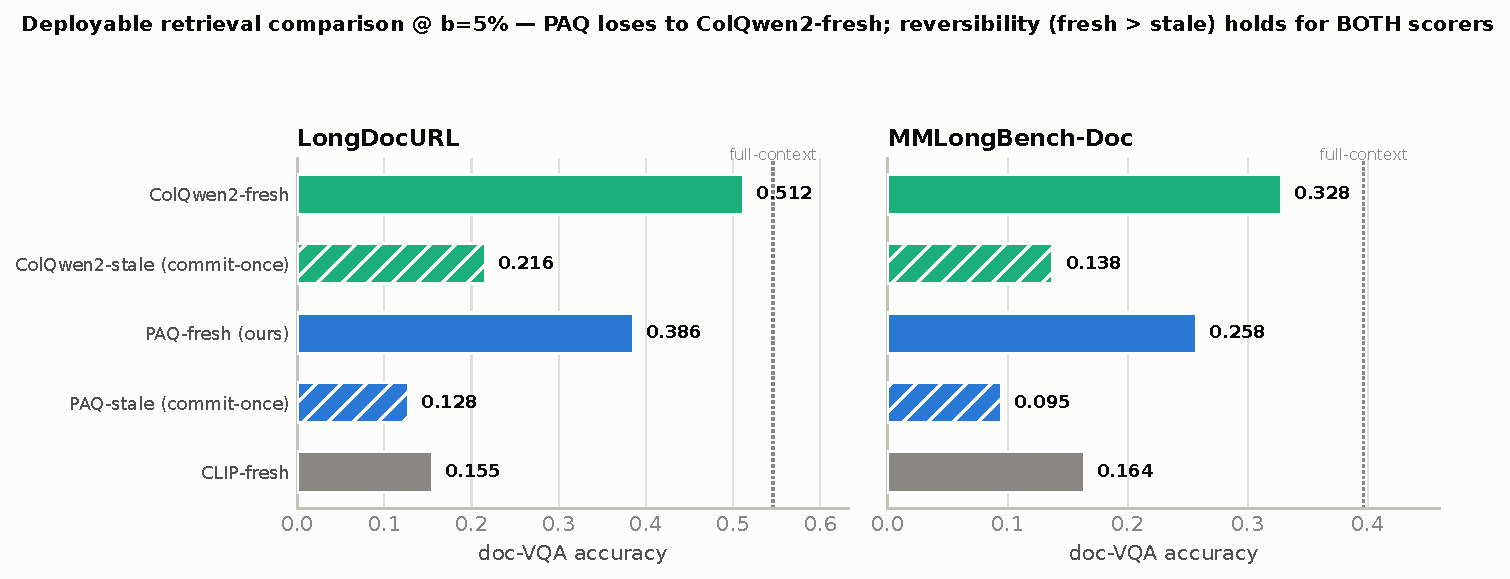
\includegraphics[width=\columnwidth]{fig_e_retrieval_reversal_light.pdf}
\caption{Two observations from the page-level system, per cell: (i) ColQwen2-fresh outperforms the page-level attention router (a loss of roughly 10 points for the router); (ii) \emph{both} scorers collapse when committed once, so reversibility is a general property of the multi-query regime rather than being scorer-specific. \paq{} here is the earlier page-level router of this appendix, not \paqc{}; the below-page \paqc{} comparison at matched budget is in Table~\ref{tab:paqkv}.}
\label{fig:retrieval}
\end{figure}

\paragraph{\paqt{}: expert-head recall and the parity accuracy evaluation.} Scoring with a single expert (layer, head) chosen by held-out-document cross-validation (CAPS's technique) lifts held-out gold-page recall@5\% to $0.683$ ($n{=}451$) / $0.626$ ($n{=}425$), meeting or exceeding ColQwen2's in-harness $0.664$/$0.536$; mean aggregation at higher scoring resolution moves almost nothing ($0.494/0.443 \to 0.500/0.452$), so the head, not the resolution, is the lever. All selected fold heads sit in layer 21. The pre-registered accuracy evaluation (bars frozen before the run; same reader, render policy, and scorer as the cached baseline rows; only the selected page set differs) lands at parity: \paqt{} $0.518$/$0.357$ vs.\ ColQwen2-fresh $0.512$/$0.328$; deltas $+0.006$ $[-0.018,+0.030]$ and $+0.028$ $[+0.001,+0.055]$; pooled $+0.017$ $[-0.000,+0.035]$. This is non-inferior under the frozen lower-bound margin ($>{-0.03}$) on both cells but not the pre-registered improvement criterion (all lower bounds $>0$), and we do not present the marginal per-cell interval as evidence of superiority. The initially better-looking complete-case verdict (pooled $+0.023$, lower bound $+0.005$) was blocked in review for informative missingness: the ${\approx}4\%$ of queries whose high-resolution scoring ran out of memory had cached baseline accuracy $0.62$, far above the cell means; a conservative reduced-resolution recovery of 31/35 missing rows (degrading only the \paqt{} arm, never the baseline) erased the pooled edge. Two caveats carry over: head selection is cross-validated \emph{benchmark-supervised} model selection (not zero-shot; the externally selected L21.H18 of the negative transfer-gate ablation later removed this caveat from the head's existence, though not from its benchmark-tuned use), and the expert-head technique is CAPS's, so the residual novelty at page level is only the amortized one-prefill-many-queries architecture.

\section{Additional Limitations Detail}\label{app:limitations-detail}
\paragraph{LongDocURL conversion-bound decomposition.} A re-analysis of the executed rows suggests the shortfall there lies largely past selection: of the 463 rows, ${\approx}39\%$ fail under both \paqc{} and the gold-page oracle (zero even when handed the native-resolution gold pages), only ${\approx}10\%$ are oracle-right/\paqc{}-wrong (the selection-capturable pool), and $2.2\%$ are \paqc{}-right/oracle-wrong, so the oracle is not a strict ceiling; that no selection method can rescue these queries is an observation about this dataset, not a general rule. Native resolution already saturates the prefill on 79/80 documents, and large documents are a flat, low-leverage half. Among pure-selection levers, only a marginal oracle-chooser union passes (lower bound $+0.003$; not deployable); only a \paqc{}${\cup}$ColQwen2 hybrid passes comfortably (lower bound $+0.061$), and we exclude it as not a standalone method. We therefore offer the dispersed-vs-conversion-bound split as a hypothesis from two datasets.

\paragraph{Base-model ceiling counts.} A large fraction of queries receive no credit even given exactly the annotated gold pages: the oracle-evidence arm scores $0$ on $317/903=35.1\%$ of confirmatory queries and a full $1$ on only $45.1\%$. Pairing controls for shared query difficulty; the oracle is not a strict ceiling (a selected page set can score above the annotated gold set on individual queries).

\paragraph{Remaining protocol caveats.} The commit-once aggregate uses the first $M{=}\min(3,k)$ queries in frozen arrival order (order-permutation and $M$-sensitivity checks remain to be run; the order-free static partially covers this), and the page-level confirmatory run predates the cache fix (\S\ref{sec:integrity}); its isolation \emph{contrasts} were verified robust, but its absolute fresh-arm levels carry ${\approx}0.04$ inflation on the 24-document check.

\end{document}
